%**************************************%
%* Generated from MathBook XML source *%
%*    on 2017-03-20T13:23:09-05:00    *%
%*                                    *%
%*   http://mathbook.pugetsound.edu   *%
%*                                    *%
%**************************************%
\documentclass[10pt,]{book}
%% Custom Preamble Entries, early (use latex.preamble.early)
%% Inline math delimiters, \(, \), need to be robust
%% 2016-01-31:  latexrelease.sty  supersedes  fixltx2e.sty
%% If  latexrelease.sty  exists, bugfix is in kernel
%% If not, bugfix is in  fixltx2e.sty
%% See:  https://tug.org/TUGboat/tb36-3/tb114ltnews22.pdf
%% and read "Fewer fragile commands" in distribution's  latexchanges.pdf
\IfFileExists{latexrelease.sty}{}{\usepackage{fixltx2e}}
%% Text height identically 9 inches, text width varies on point size
%% See Bringhurst 2.1.1 on measure for recommendations
%% 75 characters per line (count spaces, punctuation) is target
%% which is the upper limit of Bringhurst's recommendations
%% Load geometry package to allow page margin adjustments
\usepackage{geometry}
\geometry{letterpaper,total={340pt,9.0in}}
%% Custom Page Layout Adjustments (use latex.geometry)
%% This LaTeX file may be compiled with pdflatex, xelatex, or lualatex
%% The following provides engine-specific capabilities
%% Generally, xelatex and lualatex will do better languages other than US English
%% You can pick from the conditional if you will only ever use one engine
\usepackage{ifthen}
\usepackage{ifxetex,ifluatex}
\ifthenelse{\boolean{xetex} \or \boolean{luatex}}{%
%% begin: xelatex and lualatex-specific configuration
%% fontspec package will make Latin Modern (lmodern) the default font
\ifxetex\usepackage{xltxtra}\fi
\usepackage{fontspec}
%% realscripts is the only part of xltxtra relevant to lualatex 
\ifluatex\usepackage{realscripts}\fi
%% 
%% Extensive support for other languages
\usepackage{polyglossia}
\setdefaultlanguage{english}
%% Magyar (Hungarian)
\setotherlanguage{magyar}
%% Spanish
\setotherlanguage{spanish}
%% Vietnamese
\setotherlanguage{vietnamese}
%% end: xelatex and lualatex-specific configuration
}{%
%% begin: pdflatex-specific configuration
%% translate common Unicode to their LaTeX equivalents
%% Also, fontenc with T1 makes CM-Super the default font
%% (\input{ix-utf8enc.dfu} from the "inputenx" package is possible addition (broken?)
\usepackage[T1]{fontenc}
\usepackage[utf8]{inputenc}
%% end: pdflatex-specific configuration
}
%% Monospace font: Inconsolata (zi4)
%% Sponsored by TUG: http://levien.com/type/myfonts/inconsolata.html
%% See package documentation for excellent instructions
%% One caveat, seem to need full file name to locate OTF files
%% Loads the "upquote" package as needed, so we don't have to
%% Upright quotes might come from the  textcomp  package, which we also use
%% We employ the shapely \ell to match Google Font version
%% pdflatex: "varqu" option produces best upright quotes
%% xelatex,lualatex: add StylisticSet 1 for shapely \ell
%% xelatex,lualatex: add StylisticSet 2 for plain zero
%% xelatex,lualatex: we add StylisticSet 3 for upright quotes
%% 
\ifthenelse{\boolean{xetex} \or \boolean{luatex}}{%
%% begin: xelatex and lualatex-specific monospace font
\usepackage{zi4}
\setmonofont[BoldFont=Inconsolatazi4-Bold.otf,StylisticSet={1,3}]{Inconsolatazi4-Regular.otf}
%% end: xelatex and lualatex-specific monospace font
}{%
%% begin: pdflatex-specific monospace font
\usepackage[varqu]{zi4}
%% end: pdflatex-specific monospace font
}
%% Symbols, align environment, bracket-matrix
\usepackage{amsmath}
\usepackage{amssymb}
%% allow more columns to a matrix
%% can make this even bigger by overriding with  latex.preamble.late  processing option
\setcounter{MaxMatrixCols}{30}
%%
%% Color support, xcolor package
%% Always loaded.  Used for:
%% mdframed boxes, add/delete text, author tools
\PassOptionsToPackage{usenames,dvipsnames,svgnames,table}{xcolor}
\usepackage{xcolor}
%%
%% Semantic Macros
%% To preserve meaning in a LaTeX file
%% Only defined here if required in this document
%% Used for inline definitions of terms
\newcommand{\terminology}[1]{\textbf{#1}}
%% Used to markup acronyms, text or titles
%% default is small caps (Bringhurst, 4e, 3.2.2, p. 48)
%% Titles are no-ops now, see comments in XSL source
\newcommand{\acronym}[1]{\textsc{\MakeLowercase{#1}}}
\DeclareRobustCommand{\acronymintitle}[1]{\texorpdfstring{#1}{#1}}
%% Subdivision Numbering, Chapters, Sections, Subsections, etc
%% Subdivision numbers may be turned off at some level ("depth")
%% A section *always* has depth 1, contrary to us counting from the document root
%% The latex default is 3.  If a larger number is present here, then
%% removing this command may make some cross-references ambiguous
%% The precursor variable $numbering-maxlevel is checked for consistency in the common XSL file
\setcounter{secnumdepth}{3}
%% mdframed environments use a tikz frame method
\usepackage{tikz}%% Environments with amsthm package
%% Theorem-like environments in "plain" style, with or without proof
\usepackage{amsthm}
\theoremstyle{plain}
%% Numbering for Theorems, Conjectures, Examples, Figures, etc
%% Controlled by  numbering.theorems.level  processing parameter
%% Always need a theorem environment to set base numbering scheme
%% even if document has no theorems (but has other environments)
\newtheorem{theorem}{Theorem}[section]
%% Only variants actually used in document appear here
%% Style is like a theorem, and for statements without proofs
%% Numbering: all theorem-like numbered consecutively
%% i.e. Corollary 4.3 follows Theorem 4.2
%% Example-like environments, normal text
%% Numbering is in sync with theorems, etc
\theoremstyle{definition}
\newtheorem{example}[theorem]{Example}
%% Package for breakable highlight boxes
\usepackage[framemethod=tikz]{mdframed}
%% begin: assemblage
%% minimally structured content, high visibility presentation
%% environments (untitled, titled), with style
\newenvironment{assemblage-untitled}{\mdfsetup{%
roundcorner=2ex, backgroundcolor=blue!5,linecolor=blue!75!black,}%
\begin{mdframed}}{\end{mdframed}}
\newenvironment{assemblage}[1]{\mdfsetup{frametitle={\colorbox{blue!20}{\space#1\space}},%
frametitlealignment={\hspace*{1ex}}, frametitleaboveskip=-1.5ex, frametitlebelowskip=0pt,%
roundcorner=2ex, backgroundcolor=blue!5,linecolor=blue!75!black,}%
\begin{mdframed}}{\end{mdframed}}
%% end: assemblage
%% Miscellaneous environments, normal text
%% Numbering for inline exercises and lists is in sync with theorems, etc
\theoremstyle{definition}
\newtheorem{exercise}[theorem]{Exercise}
%% Localize LaTeX supplied names (possibly none)
\renewcommand*{\appendixname}{Appendix}
\renewcommand*{\chaptername}{Chapter}
%% For improved tables
\usepackage{array}
%% Some extra height on each row is desirable, especially with horizontal rules
%% Increment determined experimentally
\setlength{\extrarowheight}{0.2ex}
%% Define variable thickness horizontal rules, full and partial
%% Thicknesses are 0.03, 0.05, 0.08 in the  booktabs  package
\makeatletter
\newcommand{\hrulethin}  {\noalign{\hrule height 0.04em}}
\newcommand{\hrulemedium}{\noalign{\hrule height 0.07em}}
\newcommand{\hrulethick} {\noalign{\hrule height 0.11em}}
%% We preserve a copy of the \setlength package before other
%% packages (extpfeil) get a chance to load packages that redefine it
\let\oldsetlength\setlength
\newlength{\Oldarrayrulewidth}
\newcommand{\crulethin}[1]%
{\noalign{\global\oldsetlength{\Oldarrayrulewidth}{\arrayrulewidth}}%
\noalign{\global\oldsetlength{\arrayrulewidth}{0.04em}}\cline{#1}%
\noalign{\global\oldsetlength{\arrayrulewidth}{\Oldarrayrulewidth}}}%
\newcommand{\crulemedium}[1]%
{\noalign{\global\oldsetlength{\Oldarrayrulewidth}{\arrayrulewidth}}%
\noalign{\global\oldsetlength{\arrayrulewidth}{0.07em}}\cline{#1}%
\noalign{\global\oldsetlength{\arrayrulewidth}{\Oldarrayrulewidth}}}
\newcommand{\crulethick}[1]%
{\noalign{\global\oldsetlength{\Oldarrayrulewidth}{\arrayrulewidth}}%
\noalign{\global\oldsetlength{\arrayrulewidth}{0.11em}}\cline{#1}%
\noalign{\global\oldsetlength{\arrayrulewidth}{\Oldarrayrulewidth}}}
%% Single letter column specifiers defined via array package
\newcolumntype{A}{!{\vrule width 0.04em}}
\newcolumntype{B}{!{\vrule width 0.07em}}
\newcolumntype{C}{!{\vrule width 0.11em}}
\makeatother
%% Figures, Tables, Listings, Floats
%% The [H]ere option of the float package fixes floats in-place,
%% in deference to web usage, where floats are totally irrelevant
%% We re/define the figure, table and listing environments, if used
%%   1) New mbxfigure and/or mbxtable environments are defined with float package
%%   2) Standard LaTeX environments redefined to use new environments
%%   3) Standard LaTeX environments redefined to step theorem counter
%%   4) Counter for new environments is set to the theorem counter before caption
%% You can remove all this figure/table setup, to restore standard LaTeX behavior
%% HOWEVER, numbering of figures/tables AND theorems/examples/remarks, etc
%% WILL ALL de-synchronize with the numbering in the HTML version
%% You can remove the [H] argument of the \newfloat command, to allow flotation and 
%% preserve numbering, BUT the numbering may then appear "out-of-order"
\usepackage{float}
\usepackage[bf]{caption} % http://tex.stackexchange.com/questions/95631/defining-a-new-type-of-floating-environment 
\usepackage{newfloat}
% Figure environment setup so that it no longer floats
\SetupFloatingEnvironment{figure}{fileext=lof,placement={H},within=section,name=Figure}
% figures have the same number as theorems: http://tex.stackexchange.com/questions/16195/how-to-make-equations-figures-and-theorems-use-the-same-numbering-scheme 
\makeatletter
\let\c@figure\c@theorem
\makeatother
% Table environment setup so that it no longer floats
\SetupFloatingEnvironment{table}{fileext=lot,placement={H},within=section,name=Table}
% tables have the same number as theorems: http://tex.stackexchange.com/questions/16195/how-to-make-equations-figures-and-theorems-use-the-same-numbering-scheme 
\makeatletter
\let\c@table\c@theorem
\makeatother
%% Raster graphics inclusion, wrapped figures in paragraphs
%% \resizebox sometimes used for images in side-by-side layout
\usepackage{graphicx}
%%
%% More flexible list management, esp. for references and exercises
%% But also for specifying labels (i.e. custom order) on nested lists
\usepackage{enumitem}
%% Lists of exercises in their own section, maximum depth 4
\newlist{exerciselist}{description}{4}
\setlist[exerciselist]{leftmargin=0pt,itemsep=1.0ex,topsep=1.0ex,partopsep=0pt,parsep=0pt}
%% Support for index creation
%% imakeidx package does not require extra pass (as with makeidx)
%% Title of the "Index" section set via a keyword
%% Language support for the "see" and "see also" phrases
\usepackage{imakeidx}
\makeindex[title=Index, intoc=true]
\renewcommand{\seename}{see}
\renewcommand{\alsoname}{see also}
%% hyperref driver does not need to be specified
\usepackage{hyperref}
%% configure hyperref's  \url  to match listings' inline verbatim
\renewcommand\UrlFont{\small\ttfamily}
%% Hyperlinking active in PDFs, all links solid and blue
\hypersetup{colorlinks=true,linkcolor=blue,citecolor=blue,filecolor=blue,urlcolor=blue}
\hypersetup{pdftitle={Business Calculus with Excel}}
%% If you manually remove hyperref, leave in this next command
\providecommand\phantomsection{}
%% If tikz has been loaded, replace ampersand with \amp macro
%% extpfeil package for certain extensible arrows,
%% as also provided by MathJax extension of the same name
%% NB: this package loads mtools, which loads calc, which redefines
%%     \setlength, so it can be removed if it seems to be in the 
%%     way and your math does not use:
%%     
%%     \xtwoheadrightarrow, \xtwoheadleftarrow, \xmapsto, \xlongequal, \xtofrom
%%     
%%     we have had to be extra careful with variable thickness
%%     lines in tables, and so also load this package late
\usepackage{extpfeil}
%% Custom Preamble Entries, late (use latex.preamble.late)
%% Begin: Author-provided packages
%% (From  docinfo/latex-preamble/package  elements)
%% End: Author-provided packages
%% Begin: Author-provided macros
%% (From  docinfo/macros  element)
%% Plus three from MBX for XML characters

\newcommand{\lt}{ < }
\newcommand{\gt}{ > }
\newcommand{\amp}{ & }
%% End: Author-provided macros
%% Title page information for book
\title{Business Calculus with Excel}
\author{Mike May, S.J.\\
Department of Mathematics and Statistics\\
Saint Louis University\\
\href{mailto:maymk@slu.edu}{\nolinkurl{maymk@slu.edu}}
\and
Anneke Bart\\
Department of Mathematics and Statistics\\
Saint Louis University\\
\href{mailto:barta@slu.edu}{\nolinkurl{barta@slu.edu}}
}
\date{March 20, 2017}
\begin{document}
\frontmatter
%% begin: half-title
\thispagestyle{empty}
{\centering
\vspace*{0.28\textheight}
{\Huge Business Calculus with Excel}\\}
\clearpage
%% end:   half-title
%% begin: adcard
\thispagestyle{empty}
\null%
\clearpage
%% end:   adcard
%% begin: title page
%% Inspired by Peter Wilson's "titleDB" in "titlepages" CTAN package
\thispagestyle{empty}
{\centering
\vspace*{0.14\textheight}
%% Target for xref to top-level element is ToC
\addtocontents{toc}{\protect\hypertarget{index}{}}
{\Huge Business Calculus with Excel}\\[3\baselineskip]
{\Large Mike May, S.J.}\\[0.5\baselineskip]
{\Large Saint Louis University}\\[3\baselineskip]
{\Large Anneke Bart}\\[0.5\baselineskip]
{\Large Saint Louis University}\\[3\baselineskip]
{\Large March 20, 2017}\\}
\clearpage
%% end:   title page
%% begin: copyright-page
\thispagestyle{empty}
\vspace*{\stretch{2}}
\noindent\textcopyright\ 2012\textendash{}2017\quad{}Mike May, S.J. and Anneke Bart\\[0.5\baselineskip]

            
 

            This work is licensed under a 
          
            \href{http://creativecommons.org/licenses/by-nc-sa/4.0/}{Creative Commons Attribution-NonComercial-ShareAlike 4.0 International License}.\par\medskip
\vspace*{\stretch{1}}
\null\clearpage
%% end:   copyright-page
%% begin: acknowledgement
\chapter*{Acknowledgements}\label{acknowledgement-1}
\addcontentsline{toc}{chapter}{Acknowledgements}
This book got its start at a talk by Felkel and Richardson  at ICTCM in 2000 where they claimed "Business students should be taught math using spreadsheets."  A number of years later I tried teaching with their book and found much to appreciate from their approach.  Their book, Networked Business Mathematics, is the initial inspiration of this book.  However, as often happens when an academic looks at a textbook, I found the authors had made some choices I disagreed with, so I wanted to write my own text.  As I was going through beta versions of this book, I  discovered the 2004 report of the Curriculum Reform Across the First Two Years (CRAFTY) sub-committee of the Mathematical Association of America (MAA), and the MAA's 2004 curriculum guide.  That report has guided many decision concerning this text.
%
\par
  This year the book has been rewritten in MathBook XML (\href{http://mathbook.pugetsound.edu}{http://mathbook.pugetsound.edu}), making it possible to quickly output print, web, \acronym{PDF} versions and more from the same source.%
\par
  The continued development of my attempt to make make courses that better fit the needs of business studnets has  has received support from the National Science Foundation (Award \#DUE-16251423.)%
%% end:   acknowledgement
%% begin: preface
\chapter*{Preface}\label{preface-1}
\addcontentsline{toc}{chapter}{Preface}
This text is intended for a one semester calculus course for business students with the equivalent of a college algebra prerequisite.  Rather than being a three-semester engineering calculus course that has been watered down to fit into one semester it is designed for these students%
\par
 We assume that %
\leavevmode%
\begin{itemize}[label=\textbullet]
\item{}The student has easy access to a spreadsheet and the internet.%
\item{}This is probably the last math class the student will take.%
\item{}The student has easy access to a spreadsheet and the internet.%
\item{}The student is either majoring in business, or will use mathematics in a business setting.%
\end{itemize}
\par
This text tries to follow the recommendations of the CAFTY reports.%
\par

The MAA curriculum guide (2004) notes that many of our current math courses were designed in the last century in response to the needs of physics and engineering. One might caricaturize a standard textbook for business calculus, often called brief calculus as a watered down version of a three-semester course in calculus that was designed for physics or math majors. The main emphasis is skill in symbolic manipulation. The standard text for a one semester survey of calculus is used for both business and the life sciences. To allow for broad marketing the text is technology agnostic, follows the arrangement of a course for majors, and uses the notational conventions of mathematics.%
\par
The initial reaction from students and teachers to the text have been positive.  In particular, many report leaving the course with an understanding of how the course connects to the rest of their business curriculum%
\par
 This book remains a work in progress.  Feel free to send comments, corrections, or rebuttals.%
\par

In contrast, following the Curriculum Reform Project recommendations, a course for business calculus should:%
\leavevmode%
\begin{itemize}[label=\textbullet]
\item{}Use spreadsheets as the primary computational engine.%
\item{}Have greater emphasis on constructing mathematical models from data.%
\item{}Increase the emphasis on numerical methods rather than symbolic manipulation.%
\item{}Whenever possible use the terminology and notational conventions of the
business world.%
\item{}Consistently use examples that the students will recognize as relevant 
to the courses in their major.%
\end{itemize}
\par
 Following the CRAFTY guidelines lead to a number of subtle but pervasive shifts in a calculus text.%
\leavevmode%
\begin{itemize}[label=\textbullet]
\item{}Teaching the technology in a way that makes it portable: Experience showed, as expected, that the students would have to be taught to use Excel. Since the intent was to have the students see the material as usable outside of class, the text does not use any macros or instructor provided tools. Students are also expected to use “Good Excel Style” and make worksheets readable with sufficient documentation. 
%
\item{} Use of business terminology and conventions: Economics examples traditionally use p and q axis with q as the independent variable. In business disciplines a marginal function is not a derivative, as it is often described in calculus texts, but a difference quotient with denominator 1. %
\item{} Use of business examples: The standard textbook example for related rates is that of a person on a ladder that is sliding down a wall. One student commented that he learned to never stand on an unsecured ladder. In contrast our text uses the Cobb-Douglas equation and rate of change of revenue with respect to cost to illustrate related rates, given that both are functions of quantity. Other examples in the text include the standard supply and demand problems, marginal cost, revenue and profit problems, and present and future value of an investment. 
%
\item{} Change of order of topics: Checking with business faculty we have found that partial derivatives are considered more important than integrals. We reorder the sequence of topics to do multivariable functions and partial derivatives before integration.
%
\item{} Numerical techniques: With a spreadsheet, approximations of the derivative using the symmetric difference and Riemann sums for integration are reasonable tasks that work effectively for a wide variety of functions. The numerical examples shift from simply being theoretical underpinnings to being a practical approach. With the use of numerical techniques presented first, the main examples are introduced before the student has learned symbolic techniques. 
%
\item{} Use of CAS: Finding the current value of a revenue stream is an application of integration at the end of the course. The students know enough to set up the problem, but only have the integration techniques for solving symbolically if the stream is constant or exponential. Using simple CAS allows the focus to remain on a conceptual understanding of the problem. 
%
\item{} An increased emphasis on real data and modeling: With a spreadsheet is becomes reasonable to have students collect data from the web and to find a variety of best fitting curves. In the review of pre-calculus topics students are asked to decide which model should be expected to go with the data in a situation and then to find real data and produce an appropriate best fitting curve. 
%
\item{} Focus on communication and application: As mentioned above, the conventions of school mathematics use a terse style with one letter names like x, y, f, and g used as variable and function names to aid in symbol manipulation. If the goal is to produce work that someone else can read and understand 6 months later more descriptive variable and function names are used, and having sufficient documentation is considered part of answering the question. %
\end{itemize}
\par\hfill\begin{tabular}{l@{}}
Mike May, S.J.\\
maymk at slu.edu\\
St Louis, MO 2017
\end{tabular}\\\par
%% end:   preface
%% begin: table of contents
%% Adjust Table of Contents
\setcounter{tocdepth}{1}
\renewcommand*\contentsname{Contents}
\tableofcontents
%% end:   table of contents
\mainmatter
\typeout{************************************************}
\typeout{Chapter 1 Functions Graphs and Excel}
\typeout{************************************************}
\chapter[{Functions Graphs and Excel}]{Functions Graphs and Excel}\label{chap-1-FunctionsGraphsExcel}
\typeout{************************************************}
\typeout{Section 1.1 Linear Functions and models}
\typeout{************************************************}
\section[{Linear Functions and models}]{Linear Functions and models}\label{sec-1-1-LinearFunctionsAndModels}
Linear Functions and models%
\par
We will start this chapter with a review of linear functions. In business there are quite a few examples of linear equations. Examples include supply and demand functions. There are some standard concepts related to lines that we will review, including the slope. %
\par

Following the conventions of microeconomics, we will often use the variables p and q, for price and quantity, rather than x and y.  We will also follow the conventions of economics in treating quantity as the independent variable.  (The q-axis will be the horizontal axis.  A fast web search for supply demand equilibrium will convince you this standard usage.)%
\par
\terminology{Equations of a line}%
\par
From prior courses such as college algebra you will remember that lines can be written in several different forms. If we are given the slope and the \(y\)-intercept, the slope-intercept will be the equation of choice. If we are given a point and a slope, it might be faster if we use the point-slope form for a line. %
\begin{assemblage-untitled}\label{KindsOfLinearEquations}
\leavevmode%
\begin{table}
\centering
\begin{tabular}{ll}
\(y=m x+b\)&the slope-intercept form of a line\tabularnewline[0pt]
\(y-y_0=m(x-x_0)\)&the point-slope form of a line
\end{tabular}
\end{table}
\end{assemblage-untitled}
\par
In a business setting we are likely to use \(q\) instead of \(x\) and \(p\) instead of \(y\). %
\par
With this notation these standard equations of a line become:%
\begin{assemblage-untitled}\label{PQLinearEquations}
\leavevmode%
\begin{table}
\centering
\begin{tabular}{ll}
\(p=m q+b\)&the slope-intercept form of a line\tabularnewline[0pt]
\(p-p_0=m(q-q_0)\)&the point-slope form of a line
\end{tabular}
\end{table}
\end{assemblage-untitled}
\begin{example}[Supply and Demand Curves]\label{example-1}
 Supply and demand equations are often modeled by linear equations. The supply function is a line with a positive slope, and the demand function is a line with a negative slope.%
\leavevmode%
\begin{figure}
\centering
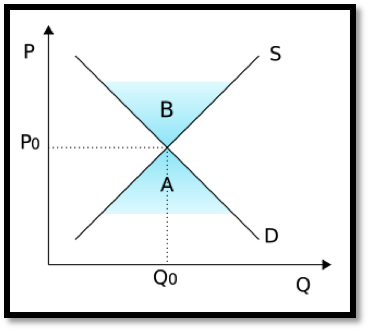
\includegraphics[width=0.5\linewidth]{images/sec1-1-SDcurves.png}
\end{figure}
\par
The vertical axis shows the price, the horizontal axis shows quantity. Both supply (S) and demand (D) are linear functions. In this diagram 'B' denotes a surplus of supply, and 'A' denotes a surplus of demand.%
\end{example}
\par



Recall, that the slope of a line through the points \(P_0=(q_0,p_0)\) and \(P_1=(q_1,p_1)\) is given by%
\begin{assemblage-untitled}\label{SlopeDef}
\begin{equation*}m=\frac{rise}{run}=\frac{(p_1-p_0)}{(q_1-q_0 )}\end{equation*}%
\end{assemblage-untitled}
\leavevmode%
\begin{figure}
\centering
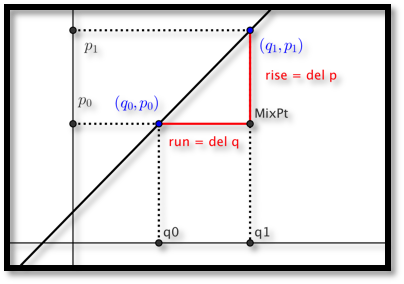
\includegraphics[width=0.5\linewidth]{images/sec1-1-slope.png}
\end{figure}
\par
There are two other forms of a line that are sometimes used. The general form of a line is a standard notation used in mathematics. The 2-point form of a line is very handy in those situations where we are not given a slope, but we are given information about two points that lie on the line.%
\begin{assemblage-untitled}\label{GeneralLinearEquations}
\leavevmode%
\begin{table}
\centering
\begin{tabular}{ll}
\(a x+b y+c=0\)& The general form of a line\tabularnewline[0pt]
\(y-y_0=(y_1-y_0)/(x_1-x_0 )(x-x_0)\) &The 2-point form of a line
\end{tabular}
\end{table}
\end{assemblage-untitled}
\par
As above, in the setting of this course we may be using \(p\) (price) and \(q\) (quantity) as our variables. This would result in equations that look as follows:%
\begin{assemblage-untitled}\label{PQGeneralLinearEquations}
\leavevmode%
\begin{table}
\centering
\begin{tabular}{ll}
\(a p+b q+c=0\)& The general form of a line\tabularnewline[0pt]
\(p-p_0=(p_1-p_0)/(q_1-q_0 )(q-q_0)\) &The 2-point form of a line
\end{tabular}
\end{table}
\end{assemblage-untitled}
\begin{example}[Finding four versions of a line]\label{example-2}

 We find that we can sell 150 widgets a day if we sell them at \textdollar{}10.  If we raise the price to \textdollar{}15, we can only sell 110 widgets a day.  Assume that there is a linear relationship between price and quantity sold.  Find the equation of the line in all four forms.%
\par

\terminology{Solution}:  Writing this using our variables p (price) and q (quantity of widgets) we see that when \(p = 10\), \(q = 150\) and when \(p = 15\), \(q = 110\).  Points are (usually) given as \((q,p)\), so this means we have two point (150,10) and (110,15) on the line. 
We always need to find the slope of the line, and in this case 
\begin{equation*}m=  \frac{5-10}{110-150}=  \frac{5}{-40}= \frac{-1}{8}\end{equation*}

We are given two points, so the 2-point form of the line should be the easiest formula to find: 
\begin{equation*}p-p_0=\frac{p_1-p_0}{q_1-q_0 }(q-q_0)\end{equation*}

We just found the slope and we just need to pick a point \((p_0,q_0)\) to finish the problem. (Recall that \(p\) and \(q\) are the variables, so we want to leave those as they are.) In this case lets pick \((p_0,q_0)= (150,10)\). Then we get this simplified version, which is also the point-slope form of this line.
\begin{equation*}p-10=\frac{-1}{8}(q-150)\end{equation*}

From here we can very easily find the slope intercept form by some straight-forward algebra:
\(p-10=\frac{-1}{8}(q-150)\) implies that 
\begin{equation*}p=\frac{-1}{8} (q-150)+10=  \frac{-1}{8} q+  \frac{150}{8}+10=  \frac{-1}{8} q+\frac{230}{8}\end{equation*}
%
\par

And finally the general form will be another exercise in algebra. We clear the fractions and put everything on one side.

\begin{equation*}8p+q-230=0.\end{equation*}%
\end{example}
\begin{example}[Finding a line from two points]\label{example-3}
  Suppose that a linear cost-quantity relationship exists in producing widgets.  There is a fixed cost of \textdollar{}400.  There is also a per-unit cost of \textdollar{}11.%
\leavevmode%
\begin{enumerate}[label=(\alph*)]
\item\hypertarget{li-18}{}Find the equation of the line.%
\item\hypertarget{li-19}{}Find the cost of making 200 widgets.%
\end{enumerate}
\par
\terminology{Solution}:%
\par
 1) We have one point of the form (quantity, cost) at (0, 400) from the fixed cost.  This point happens to be an intercept.  The slope of the line is \(m=11/1=11\).  We will let \(C\) stand for Cost and \(q\) stand for quantity. The general formula for a line with these variables will have the form
\begin{equation*}C=m q+b.\end{equation*}%
\par
In this example \(m = 11\) and \(b = 400\), hence the equation of the line is
\begin{equation*}C=11 q+400\end{equation*}%
\par
b) Using the equation form part a) we see that the cost of producing 200 widgets is
\begin{equation*}C=11 (200)+400=2,600\end{equation*}
%
\end{example}
\begin{example}[A nonlinear functions]\label{example-4}

Example 4:  Sarah is paid \textdollar{}500 for working up to 40 hours per week.  For work beyond 40 hours per week she is paid \textdollar{}18/hour.%
\leavevmode%
\begin{enumerate}[label=(\alph*)]
\item\hypertarget{li-20}{}Find the equation of the line.%
\item\hypertarget{li-21}{}How much is she paid if she works 56 hours in a week?%
\item\hypertarget{li-22}{}What is she paid for working 30 hours in a week?%
\end{enumerate}
\par
\terminology{Solution}:%
\par
	a) For this example we will use “designer variables”. The output will be Pay, and the input variable – the number of hours worked – will be hrs. We are told that Pay = 500 when hrs = 40. The slope of the line work beyond 40 hours is \(m=18\).  Another way to think of this is to say that there is a fixed Pay of \textdollar{}500 and a variable Pay for any hours in excess of 40: i.e. (hrs - 40). Thus, the equation of the line, according to the point-slope form is 
                    \begin{assemblage-untitled}\label{PayEquations}
\begin{equation*}Pay=variable\  pay+Fixed\  pay.\end{equation*}%
\end{assemblage-untitled}



\begin{equation*}Pay=m(hrs-40)+500=18*(hrs-40)+500.\end{equation*}%
\par
b) The pay for working 56 hours is 18(56-40)+500=\textdollar{}788.%
\par
c) The pay for working 30 hours is \textdollar{}500.  This is a trick question part of the problem.  From the text of the problem, the linear model only works for overtime, with a flat rate applying to less than 40 hours per week.
Comment: The function should be written as a piecewise defined function.%
\par
This question is all about the function \(f\) defined by \begin{equation*}Pay=\begin{cases}
500&hrs\le 40\\
18*(hrs-40)+500&hrs>40\\
\end{cases}\end{equation*}%
\end{example}
\par
It can be useful when writing reports to have variables that convey some meaning. We could have called \(Pay\) `\(y\)', and \(hrs\) `\(x\)', but using the much more easily interpreted variables named Pay and hrs helps when using the formulas.
%
\typeout{************************************************}
\typeout{Exercises 1.1.1 Exercises 1.1 Linear Functions and models}
\typeout{************************************************}
\subsection[{Exercises 1.1 Linear Functions and models}]{Exercises 1.1 Linear Functions and models}\label{exercises-set-sec-1-1}
For problems 1-6, given two points in the \((q,p)\) plane and a value \(q_0\):%
\leavevmode%
\begin{enumerate}[label=(\alph*)]
\item\hypertarget{li-23}{}Find the slope of the line determined by the points.%
\item\hypertarget{li-24}{}Give the equation of the line determined by the points.%
\item\hypertarget{li-25}{}Give the value of \(p\) predicted for \(q_0\) by the line.%
\end{enumerate}
\begin{exerciselist}
\item[1.]\hypertarget{exercise-1}{} 
Points \((2,5)\) and \((6,17)\), with \(q_0=4\).
%
\par\smallskip
\par\smallskip
\noindent\textbf{Hint.}\hypertarget{hint-1}{}\quad
Find the slope and use the point-slope form%
\par\smallskip
\noindent\textbf{Solution.}\hypertarget{solution-1}{}\quad
\leavevmode%
\begin{enumerate}[label=(\alph*)]
\item\hypertarget{li-26}{}First find the slope: \(m=  \frac{\text{change in }p}{\text{change in }q}
=  \frac{17-5}{6-2}=\frac{12}{4}=3\)%
\item\hypertarget{li-27}{}Next we find the equation of the line. There are several ways to do this and two methods are outlined below.%
%
\begin{itemize}[label=\textbullet]
\item{}Method 1: use the point-slope equation: \(p-p_0=m (q-q_0)\).
We can choose either one of the points, so in this case we will find the line using the point \((q_0,p_0 )=(2,5)\). This gives the equation
\(p-5=3 (q-2)\).%
\par
Rewrite this as \(p=3q-1\)%
\item{}Method 2: use the slope- intercept equation \(p=m q+b\).
Use \((q,p)=(2,5)\) and \(m = 3\) and solve for \(b\):
\(5=3 (2)+b\).
And solving for \(b\) we have that \(b= -1\), and hence \(p=3q-1\)%
\end{itemize}
\item\hypertarget{li-30}{}Evaluate at the given point.  \(p(4)=3*4-1=11\)%
\end{enumerate}
\item[2.]\hypertarget{exercise-2}{} Points \((5,7)\) and \((10,7)\), with \(q_0=20\).
%
\par\smallskip
\item[3.]\hypertarget{exercise-3}{} Points \((20,10)\) and \((40,5)\), with \(q_0=12\).
%
\par\smallskip
\par\smallskip
\noindent\textbf{Solution.}\hypertarget{solution-2}{}\quad
Just as in problem 1 we find the slope and then find the equation of the line.%
\leavevmode%
\begin{enumerate}[label=(\alph*)]
\item\hypertarget{li-31}{}First find the slope: \(m=  \frac{\text{change in }p}{\text{change in }q}
=  \frac{5-10}{40-20}=-\frac{5}{20}=-\frac{1}{4}\)%
\item\hypertarget{li-32}{}Using \(p=m (q-q_0)+p_0\) with \((q_0,p_0 )=(20, 10)\) and \(m = -\frac{1}{4}\), we get \(p=-\frac{1}{4}(q-20)+10\).  Solving for \(p\) we get \(p =-\frac{1}{4}q+15\)%
\item\hypertarget{li-33}{}Evaluate at the given point.  \(p(12)=-\frac{1}{4}(12)+15=12\)%
\end{enumerate}
\item[4.]\hypertarget{exercise-4}{} Points \((5,62)\) and \((115,783)\), with \(q_0=415\).
%
\par\smallskip
\item[5.]\hypertarget{exercise-5}{} Points \((273,578)\) and \((412,6)\), with \(q_0=309\).
%
\par\smallskip
\par\smallskip
\noindent\textbf{Solution.}\hypertarget{solution-3}{}\quad
Just as in problem 1 we find the slope and then find the equation of the line.%
\leavevmode%
\begin{enumerate}[label=(\alph*)]
\item\hypertarget{li-34}{}First find the slope: \(m=  \frac{\text{change in }p}{\text{change in }q}
=  \frac{578-6}{273-412}=-\frac{5}{20}=-\frac{572}{139}\)%
\item\hypertarget{li-35}{}Using \(p=m (q-q_0)+p_0\) with \((q_0,p_0 )=(412, 6)\) and \(m = -\frac{572}{139}\), we get \(p=-\frac{572}{139}(q-412)+6\).  (We can combine the constant terms – the \(6\) and the \(-\frac{572}{139}*(-412)\), but leaving the equation in this form is acceptable.)%
\item\hypertarget{li-36}{}Evaluate at the given point.  \(p(309)=-\frac{572}{139}(309-412)+6
=-\frac{572}{139}(-103)+6=429\frac{119}{139}\)%
\end{enumerate}
\item[6.]\hypertarget{exercise-6}{} Points \((509,17)\) and \((211,132)\), with \(q_0=4\).
%
\par\smallskip
\par
For problems 7-12, start with the information given:%
\leavevmode%
\begin{enumerate}[label=(\alph*)]
\item\hypertarget{li-37}{}Give the equation of the line determined by that information.%
\item\hypertarget{li-38}{}Give the value of predicted for \(q_0\) by the line.%
\item\hypertarget{li-39}{}Give the value of \(q\) for which the predicted value of \(p\) is \(0\).%
\end{enumerate}
\item[7.]\hypertarget{exercise-7}{} A slope of \(3\), passing through \((6,3)\), with \(q_0=4\).
%
\par\smallskip
\item[8.]\hypertarget{exercise-8}{} A slope of \(-2\), passing through \((2,-5)\), with \(q_0=3\).
%
\par\smallskip
\item[9.]\hypertarget{exercise-9}{} A slope of \(12.7\), passing through \((22,183)\), with \(q_0=46\).
%
\par\smallskip
\item[10.]\hypertarget{exercise-10}{} A slope of \(-0.23\), passing through \((7.6,19.7)\), with \(q_0=59.6\).
%
\par\smallskip
\item[11.]\hypertarget{exercise-11}{} A slope of 0, passing through \((12.3,9.8)\), with \(q_0=74\).
%
\par\smallskip
\item[12.]\hypertarget{exercise-12}{} A slope that is undefined, passing through \((6,3)\), explaining why part b would not make sense.
%
\par\smallskip
\par
For problems 13-18, start with the equation given:%
\leavevmode%
\begin{enumerate}[label=(\alph*)]
\item\hypertarget{li-40}{}Give the slope of the line or say that the slope is undefined.%
\item\hypertarget{li-41}{}Give the intercepts of the line with the axes.%
\item\hypertarget{li-42}{}Give two points that are on the line but not on the axes.%
\end{enumerate}
\item[13.]\hypertarget{exercise-13}{} \(3 p+2 q=6\).
%
\par\smallskip
\item[14.]\hypertarget{exercise-14}{} \(7 p-4 q+14=0\).
%
\par\smallskip
\item[15.]\hypertarget{exercise-15}{} \(y=5\).
%
\par\smallskip
\item[16.]\hypertarget{exercise-16}{} \(x=3\).
%
\par\smallskip
\item[17.]\hypertarget{exercise-17}{}
 \(p=4(x-3)+9\).
%
\par\smallskip
\item[18.]\hypertarget{exercise-18}{}
 \(112 p+257 q=4783\).
%
\par\smallskip
\item[19.]\hypertarget{exercise-19}{}
 Suppose that the relationship between price and quantity of widgets sold is linear.  When the price is \textdollar{}23, we can sell 4783 widgets.  If we raise the price to \textdollar{}27, we can only sell 4295 widgets.  Find the equation of the line.
%
\par\smallskip
\item[20.]\hypertarget{exercise-20}{}
 Suppose that the relationship between price and quantity of gizmo kits we can buy is linear.  When the price is \textdollar{}15, we can buy 6000 gizmo kits.  If we lower the price we will pay to \textdollar{}13, we can only buy 4500 kits.  Find the equation of the line.
%
\par\smallskip
\end{exerciselist}
\typeout{************************************************}
\typeout{Section 1.2 Functions in the Business setting}
\typeout{************************************************}
\section[{Functions in the Business setting}]{Functions in the Business setting}\label{sec-1-2-FunctionsBusinessSetting}


	Not all functions we encounter in a business setting are linear. There are several other families of functions we should (re-) familiarize ourselves with. These models include:\leavevmode%
\begin{itemize}[label=\textbullet]
\item{}	Quadratic functions%
\item{}	Exponential functions%
\item{}	Logistic Functions%
\item{}	Normal distribution functions%
\item{}	Sinusoidal functions%
\end{itemize}
%
\par
\terminology{Quadratic Functions}%
\par
\terminology{Quadratic functions} should be very familiar from previous mathematics courses. They are of the form \(y=a x^2+b x+c\). These are our standard parabolas.%
\par
In business we encounter quadratic equations when we study revenue and profit functions. Recall from your economics course that:
\begin{equation*}Revenue=price*quantity=p*q\end{equation*}
In some of the models we will investigate later in the course price will be a linear function. We will assume \(Price=m q+b\). This implies that 
\begin{equation*}Revenue=(m q+b)*q=m q^2+b q\end{equation*}
If \(m > 0\), then the revenue function will look like a parabola that opens up. If \(m \lt 0,\) then the revenue function will look like a parabola that opens down.
%
\leavevmode%
\begin{figure}
\centering
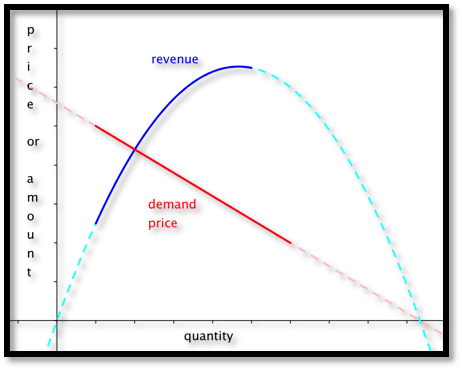
\includegraphics[width=0.5\linewidth]{images/sec1-2-QuadraticFunctions.png}
\end{figure}
\par
For a quadratic model we are often very interested in the coordinates of the vertex, and any possible zeros. For the general equation \(y=a x^2+b x+c\) the sign of the coefficient of \(x^2\), \(a\), will determine if we have a maximum or a minimum. If \(a\) is positive, the parabola opens up and the vertex will be a minimum. If \(a\) is negative, the parabola opens down and the vertex will be a maximum.%
\par

Recall that we can find the zeros of a quadratic by using the quadratic equation.
\begin{equation*}roots or zeroes  =  
\frac{-b\pm\sqrt{b^2-4ac}}{2a}\end{equation*}
From this equation we see that the vertex must be located at \(x= -b/(2a.)\). The discriminant (the term underneath the radical sign determines if there are 0, 1, or 2 roots.%
\leavevmode%
\begin{itemize}[label=\textbullet]
\item{}If \(b^2-4ac>0\), then there are 2 roots.%
\item{}If \(b^2-4ac=0\), then there is 1 root (the vertex will touch the axis)%
\item{}If \(b^2-4ac\lt 0\), then there are no roots. This means the entire graph must lie above the \(x\)-axis (\(a > 0\)) or below the \(x\)-axis (\(a \lt 0\)).%
\end{itemize}
\par

Sometimes we may need more general polynomials in a model, with an equation of the form \(f(x)=a_n x^n+\cdots+a_1 x+a_0\).  In such cases we remember that the number of turning points of the graph can be no more than \(n-1\)%
\par
\terminology{Exponential functions}%
\par
The \terminology{exponential model}, with an equation of the form \(f(t)=p*r^t\). Sometimes the exponential function \(e^t\) is denoted by \(exp(t)\). Excel will use this format, so it is worth looking at the notation in this case. 
\(f(t)=p*e^{rt}\) can also be written as  \(f(t)=p*exp(r t)\)%
\par
Math books (and Excel) like using a base of \(e\) because it makes the mathematics easier when we do calculus, so the equation is written as \(f(t)=p*e^{rt}\) or \(f(t)=p*exp(r t)\). However, in real world applications we tend to use \(A=pR^t\) and make the equation \(f(t)=p*R^t\).  (The reader is warned that \(R=e^r\) and both \(R\) and \(r\) are referred to as the \terminology{rate}.  You will have to use the context to tell them apart.)%
\par
Exponential functions are used for proportional growth or decay.  In business, compound interest is given as an exponential function. In particular, if \(P\) is the principal and \(r\) is the interest rate (expressed as a decimal), then the amount \(A\) after time \(t\) is given by \(A=P e^rt\). The relationship (in general) between a \terminology{future value} (FV) and the \terminology{present value} (PV) given an interest rate \(r\), and \(t\) being the number of compounding periods is given by:%
\begin{assemblage-untitled}\label{FutureValueDef}
\begin{equation*}Future Value: FV=PV*(1+r)^t\end{equation*}%
\end{assemblage-untitled}
\par
It is also useful in determining a fair value today of a promised future payout. The sign of the rate will determine if the graph turns up or down.%
\par
When modeling real world behavior, we often know some special features of the problem. For instance, we may know that our present value is \textdollar{}2,000 and that we would like the future value to be \textdollar{}10,000 after 10 years. The question would be what function would describe such a model? A method commonly used to solve such a problem is to plug in the values we are given and see if we can determine what the remaining quantities should be. We know that \(FV=PV*(1+r)^t\). The extra information tells us PV = 2000, and when t = 10 we know that \(FV=2000*(1+r)^{10}=10,000\).
This is enough information to solve for r. Dividing both sides by 2000 shows that \((1+r)^{10}=5\). To solve this equation we need rules of exponents. We obtain: 
\(1+r=5^{1⁄10}\), and hence \(r= 5^{1/10}-1= 0.1746\). This means that to obtain such a growth we would need a rate of growth of about 17.46\%. The function modeling that growth would be \(FV=2000*(1.1746)^t\).
In general we can set up equations and solve for the unknown quantities. 
%
\par
\terminology{Logistic Functions}%
\par

The exponential model assumes growth without end.  That is impossible in most business situation.  Instead there is typically a point where the market is saturated.  The alternative model says that the rate of change is proportional both to the current quantity and to the distance from the theoretical maximum value.  This is called logistic growth.  A typical formula for \terminology{logistic growth} given an interest rate \(r\), market saturation point \(M\), and constant a depending on the problem is%
\begin{equation*}f(x)=  \frac{M}{1+a e^{-rx}} \end{equation*}\par
In Excel we would write this function as: f(x)=M/(1+a exp(-r x)). Using Excel it is fairly easy to create a table and graph a logistic function.%
\leavevmode%
\begin{figure}
\centering
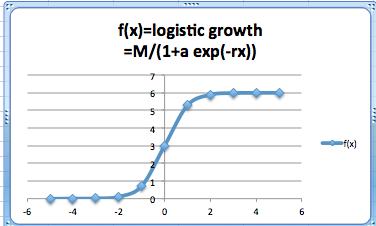
\includegraphics[width=0.5\linewidth]{images/sec1-2-LogisticFunction.png}
\end{figure}
\par
\terminology{Sinusoidal Functions}%
\par
The \terminology{sinusoidal model} is for data that repeats on a natural cycle.  Typical examples would include need for heating oil, electricity for air conditioning, and sales for seasonal items such as Christmas.  The typical equation is
%
\begin{equation*}f(x)=M+A*sin(2\pi*(x+shift)/period),\end{equation*}\par

where the mean \(M\) is the average value, the amplitude \(A\) is the distance from the mean to the maximum, the period is the length of time till the cycle repeats, and the shift is where we start the cycle for \(x=0\).  
With an appropriate shift we can interchange the sine and cosine functions.  (The functions \(sin(x)\) and \(cos(x)\) arise from trigonometry.)  In this course, we will not focus on trigonometric functions and their properties.  We are only concerned with having a periodic function for seasonal variations.%
\leavevmode%
\begin{figure}
\centering
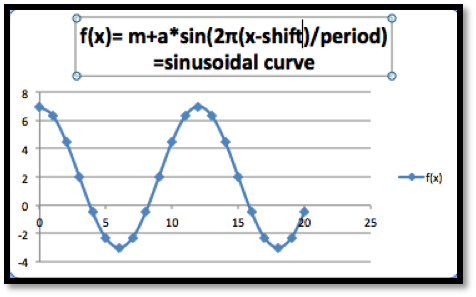
\includegraphics[width=0.5\linewidth]{images/sec1-2-SinCurve.png}
\end{figure}
\par
\terminology{Normal distribution Functions}%
\par
The \terminology{normal distribution} or \terminology{bell curve} is used because many populations follow a normal distribution on many scales.  The equation%
\begin{equation*}f(x)=a e^{\left(\frac{-(m-x)}{s}\right)^2} \end{equation*}\par

looks a bit intimidating, but we will be able to use the power of a spreadsheet to easily handle it. %
\par
In retail, there are several examples of items that follow a normal distribution. In a store selling shoes for women for instance, we would expect to see that some sizes are more prevalent than others. This would be a factor in determining what sizes to have in stock, and at what quantities. 
The typical scenario in which we will be using this curve model is one where we ask what range of sizes do we need to cover for the population in an area to be large enough to justify a specialty store.%
\leavevmode%
\begin{figure}
\centering
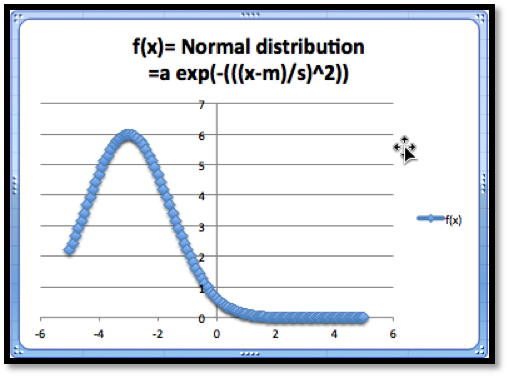
\includegraphics[width=0.5\linewidth]{images/sec1-2-NormalCurve.png}
\end{figure}
\par
The normal distribution function has certain interesting features. The graph shows a maximum value. The maximum occurs when \(x = m\). And when \(x = m\), we know that %
\begin{equation*}f(x)=a e^{\left(\frac{-(m-m)}{s}\right)^2}=a e^0=a*1=a,\end{equation*}\par
 hence the maximum value is \(a\).%
\par
There are a few more models that will show up from time to time and are worth mentioning.%
\par

\terminology{Inversely proportional Functions}%
\par
If we see the phrase that two quantities are inversely proportional, it means that \(f(x)\) is a constant times \(1/x\).  We might expect to use such a model when a fixed amount of money will be spent to acquire all of a given product.  Thus we may see it used to describe price as a function of supply.%
\leavevmode%
\begin{figure}
\centering
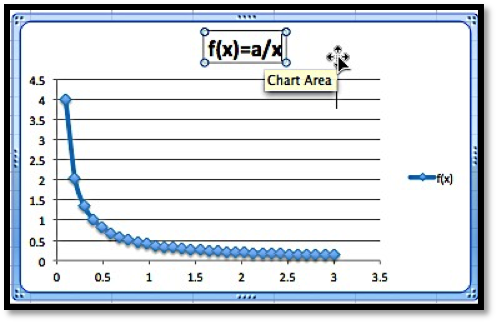
\includegraphics[width=0.5\linewidth]{images/sec1-2-InverseCurve.png}
\end{figure}
\par

\terminology{Logarithmic Functions}%
\par
The \terminology{logarithmic model} looks at equations of the form \(f(x)=a*ln(x)\).  This model shows up in two ways.  It can be obtained as the accumulation of a quantity that is inversely proportional to our variable.  It also shows up as the inverse of the exponential model.  (If \(y\) is described as an exponential function of \(x\), then \(x\) is a logarithmic function of \(y\).)%
\leavevmode%
\begin{figure}
\centering
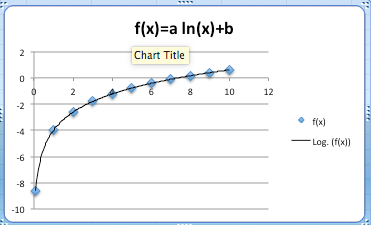
\includegraphics[width=0.5\linewidth]{images/sec1-2-LogCurve.png}
\end{figure}
\typeout{************************************************}
\typeout{Exercises 1.2.1 Exercises  Functions in the Business Setting}
\typeout{************************************************}
\subsection[{Exercises  Functions in the Business Setting}]{Exercises  Functions in the Business Setting}\label{exercises-set-sec-1-2}
For each model, some features of the graph are listed.  Describe how to change each feature by changing the parameters of the model.  (E.g., With the linear model, 
\(f(x)=a x+b\), the parameters are \(a\) and \(b\).  The place where the line intercepts the 
\(x\)-axis is \(–b/a\), so any \(x\)-intercept can be produced with \(a=-1\) and \(b\) equal to the desired value.)%
\begin{exerciselist}
\item[1.]\hypertarget{exercise-21}{} For a linear model, \(f(x)=a x+b\), how do I get a graph with 
\leavevmode%
\begin{enumerate}[label=(\alph*)]
\item\hypertarget{li-51}{}A positive \(y\)-intercept?%
\item\hypertarget{li-52}{}A negative slope?%
\end{enumerate}

%
\par\smallskip
\item[2.]\hypertarget{exercise-22}{} Suppose we are working with a quadratic model, \(f(x)=a x^2+b x+c\)
\leavevmode%
\begin{enumerate}[label=(\alph*)]
\item\hypertarget{li-53}{}How do we get a graph, that points down? (i.e. a graph that has a maximum)?%
\item\hypertarget{li-54}{}How will we know if the graph of the function intercepts the \(x\)-axis at two positive values?%
\end{enumerate}

%
\par\smallskip
\item[3.]\hypertarget{exercise-23}{} For a quadratic model, \(f(x)=a x^2+b x+c\), How do I get a graph where the vertex has \(x=5\)?
%
\par\smallskip
\item[4.]\hypertarget{exercise-24}{} For a polynomial model, \(f(x)=a_n x^n+\cdots+a_1 x+a_0\), how do I get a graph that goes up at both ends?
%
\par\smallskip
\item[5.]\hypertarget{exercise-25}{} For an exponential model, \(f(x)=P*\exp(r x)\), how do I get a graph with \(f(0)=100\), that goes to zero as x gets large?
%
\par\smallskip
\item[6.]\hypertarget{exercise-26}{} For an exponential model, \(f(x)\exp(-r t)\), how do I get a graph where \(f(x)\) goes to 10 as \(x\) gets large, \(f(0)=1\), and \(f(10)\) is at least \(9\)?
%
\par\smallskip
\item[7.]\hypertarget{exercise-27}{} For a sinusoidal model, \(f(x)=M+A \sin(2\pi(x+shift)/period)\), based on seasonal change through the year, if \(x\) is measured in months, what value should period have?
%
\par\smallskip
\item[8.]\hypertarget{exercise-28}{} For a normal model, 
\(f(x)=a \exp\left(-\left(\frac{x-m}{s}\right)^2\right)\), how do I produce a graph with a high point at \((7, 20)\), and the value of \(f(4)\) between 1 and 2?  (You need to use trial and error on this problem.)
%
\par\smallskip
\item[9.]\hypertarget{exercise-29}{} For a normal model, 
\(f(x)=a \exp\left(-\left(\frac{x-m}{s}\right)^2\right)\), how do I produce a graph with a high point at \((7, 20)\), and the value of \(f(1)\) between 1 and 2?  (You need to use trial and error on this problem.)
%
\par\smallskip
\item[10.]\hypertarget{exercise-30}{} For the power model, \(f(x)=a x^b\), how do I produce a graph with \(f(1)=5\) and \(f(3)=1\)?%
\par\smallskip
\item[11.]\hypertarget{exercise-31}{} For the inversely proportional model, \(f(x)=a/x\), how do I produce a graph with \(f(1) \lt 0\) and \(f(3)=-5?\)%
\par\smallskip
\item[12.]\hypertarget{exercise-32}{} For the logarithmic model, \(f(x)=a \ln(x)\) how do I produce a graph with \(f(e)=3\)?%
\par\smallskip
\par
Exercises 14-21) For each situation, explain which model you would use for each situation (linear, quadratic, etc.).  Be sure to explicitly mention what you are using as the free variable (the equivalent of x), what you are using as the dependent variable (the equivalent of y), and why that model makes sense in the given situation.%
\item[13.]\hypertarget{exercise-33}{} The cost of producing an amount of a product is the sum of the fixed costs, like warehouse rent, and the variable costs, like labor and materials, which we can assume to be the same for each unit produced.
%
\par\smallskip
\item[14.]\hypertarget{exercise-34}{} When looking at revenue, we can assume that sales will be linear function of the price of the object.
%
\par\smallskip
\item[15.]\hypertarget{exercise-35}{} The amount I expect to be able to withdraw from an account at a future date, assuming that interest is compounded continuously and is fixed.
%
\par\smallskip
\item[16.]\hypertarget{exercise-36}{} The amount of time it takes an investment to double assuming a fixed interest rate.
%
\par\smallskip
\item[17.]\hypertarget{exercise-37}{} The amount of electricity needed for air conditioners in a Washington, D.C. at various times of the year.
%
\par\smallskip
\item[18.]\hypertarget{exercise-38}{} The amount of metal needed to build a fuel tank as a function of the amount of fuel to be stored.
%
\par\smallskip
\item[19.]\hypertarget{exercise-39}{} The total length of booms needed to contain an oil spill as a function of the size of the spill.
%
\par\smallskip
\item[20.]\hypertarget{exercise-40}{} The monthly sales of a hot new electronic device in a country.%
\par\smallskip
\item[21.]\hypertarget{exercise-41}{} The distribution of sales of pairs of pants by leg length.%
\par\smallskip
\end{exerciselist}
\typeout{************************************************}
\typeout{Section 1.3 Introduction to Excel Spreadsheets}
\typeout{************************************************}
\section[{Introduction to Excel Spreadsheets}]{Introduction to Excel Spreadsheets}\label{sec-1-3-IntroExcelSpreadsheets}
This book will rely heavily upon the use of Excel, since it is the standard mathematical tool used in the business world.  (More precisely, the spreadsheet is the standard tool, and Excel is currently the de facto standard brand.  Most of this text can easily be used with other spreadsheets.) However, we do not assume that the student has worked with Excel previously. Throughout the course we will introduce those features of Excel we need to do mathematics and model the business problems we encounter.
%
\par

While introducing Excel, we will also introduce rules of “Good Excel practice.”  In a business environment, spreadsheets should be written so that someone else can easily understand the worksheet, and maintain it for future use. You should assume those same standards when submitting work in Excel.
%
\par
This section is meant as an introduction to several standard features of Excel we will use often. These include:
%
\leavevmode%
\begin{itemize}[label=\textbullet]
\item{}
\terminology{Basic Arithmetic} such as add, subtract, multiply etc.
%
\item{}
\terminology{Show formulas}: allows us to check if the formulas in the cells are what they should be.
%
\item{}
\terminology{Quick fill}: this feature takes a pattern and fills it across a column or a row.
%
\item{}
\terminology{Relative and Absolute Reference}: when do we refer to a fixed cell and when does the reference depend on our place in the spreadsheet? 
%
\item{}
\terminology{SUM()}: Adding a large number of cells can be efficiently done with this feature.
%
\end{itemize}
\par

\terminology{Basic Arithmetic, show formulas and quick fill.}%
\par
We start with an example that covers basic arithmetic.  Assume we are given the following worksheet:
%
\leavevmode%
\begin{figure}
\centering
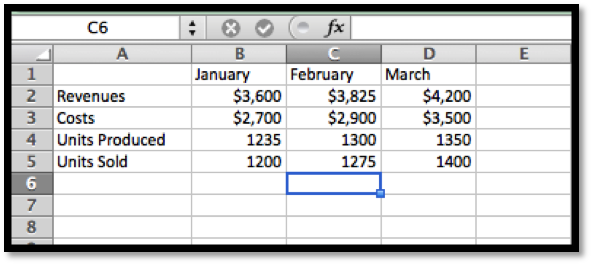
\includegraphics[width=0.5\linewidth]{images/sec1-3-1BasicData.png}
\end{figure}
\par
From data we would like to compute the figures for the quarter (add the three months), the monthly profit (revenues-cost), and the monthly unit costs (costs/ units sold).%
\par

With the formula ribbon, we go to show and select \terminology{Show Formulas}.  Since we want the worksheet to be readable by others, we add labels for the quantities we are computing, and in each cell we enter the formula for the quantity.   The formula bar tells us which cell has been selected and the formula for that cell.   It is generally easier to edit a formula by using the formula bar.%
\par
In this example, we have used several different ways of writing the formula.  In cells E2, B6, and B7 we simply typed in the equation like we would on a calculator.  Thus the profit for January is Revenues – Costs, or 3600-2700.  Since we want Excel to compute this value, we put an equals sign at the start of the formula. %
\par
 
In cells E3, C6 and C7, instead of typing the values, we use a reference to the cell where the value is kept.  This allows us to change the raw data and have Excel automatically recompute the quantities that were derived from those numbers.%
\par

In cells E5 and E6 we use Excel's sum command.  In Cell E4, we are taking the sum of the values in the cells from B4 through D4.  We will come back to commands in Excel later in the section.%
\leavevmode%
\begin{figure}
\centering
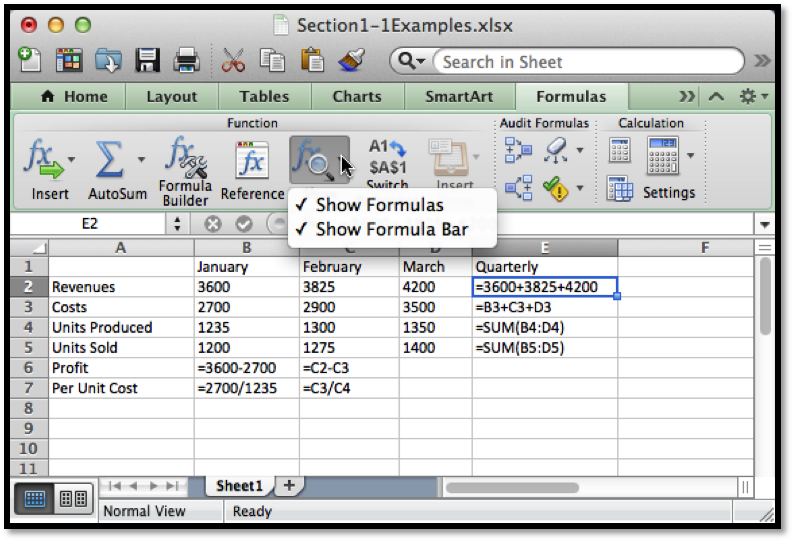
\includegraphics[width=0.8\linewidth]{images/sec1-3-2ShowFormulas.png}
\end{figure}
\par
If we unselect \terminology{Show Formulas}, we see the values that Excel computes.%
\leavevmode%
\begin{figure}
\centering
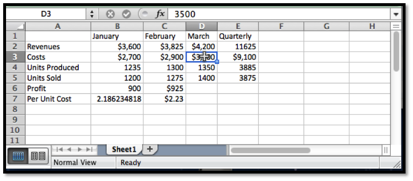
\includegraphics[width=0.8\linewidth]{images/sec1-3-3UnshowFormulas.png}
\end{figure}
\par
We want to finish our assignment by computing the Profit and Per Unit Costs for March and for the Quarter.  However, we would prefer not to type any more formulas.  (Typing in four more cells is not so bad, but we can imagine being told to do this for several years of data.)  We will use a process called Quick Fill, that tells Excel to repeat the same formula, with the cell references appropriately modified.%
\par

To do the quick fill, we select the cells we want copied.
%
\leavevmode%
\begin{figure}
\centering
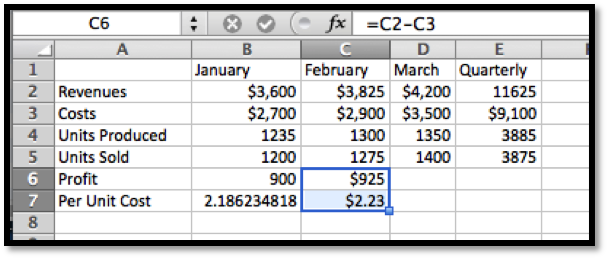
\includegraphics[width=0.8\linewidth]{images/sec1-3-4.png}
\end{figure}
\par

We can move the cursor until the cell(s) show the fill handle. This will change the symbol in the corner of the cell to a thin dark '+'.%
\leavevmode%
\begin{figure}
\centering

\includegraphics[width=0.2\linewidth]{images/sec1-3-5.png}
\end{figure}
\par
 
We then drag the little blue box at the lower left corner of the box of selected cells.  Excel automatically fills in the new values.%
\leavevmode%
\begin{figure}
\centering
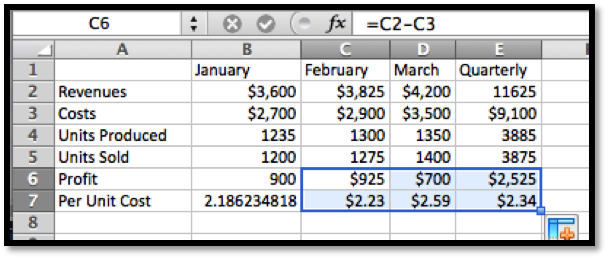
\includegraphics[width=0.8\linewidth]{images/sec1-3-6FebSums.png}
\end{figure}
\par

We look back at the formulas and see that Excel has produced formulas where cells are in the same relative position.  Profit is the value from the cell 4 rows higher minus the value of the cell three rows higher.%
\leavevmode%
\begin{figure}
\centering
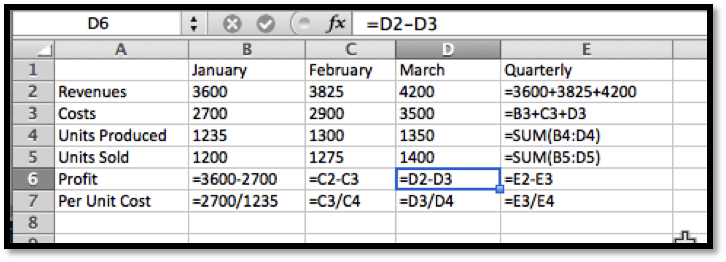
\includegraphics[width=0.8\linewidth]{images/sec1-3-7MoreSums.png}
\end{figure}
\par

There is a last detail to fix in our report.  The quantities in profit and Per Unit Cost are in money, so we want them formatted correctly.  (They should start with a dollar sign, have a decimal point, and stop at two decimal places or cents.)  We do this by selecting the cells and then formatting the cells as currency.%
\leavevmode%
\begin{figure}
\centering
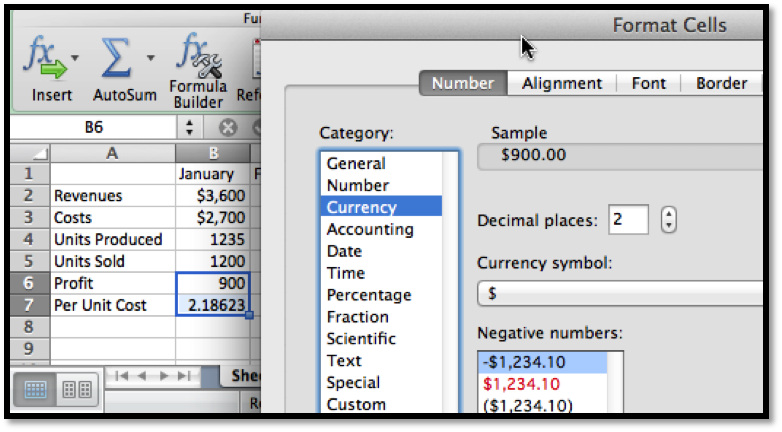
\includegraphics[width=0.8\linewidth]{images/sec1-3-8.png}
\end{figure}
\par

If we use the quick fill on a pair of numbers, Excel produces an arithmetic sequence.  A pair of cells containing 1 then 4 becomes the start of a sequence 1, 4, 7, 10,  … .%
\par
\terminology{
Absolute and Relative Cell References}%
\par

One of the reasons that spreadsheets are so useful for doing mathematics in a business setting is that businesses often do a relatively simple computation for a large number of cases.  That means we should pay attention to formulas with cell references and the process of copying a formula from one case to another.  In the example above, all of the values change from one month to the next.  It is not hard to imagine a calculation where some values remain the same for many cases.  Thus we want to look at the idea of absolute and relative cell references.  This is a very important topic and an Excel feature we will be using for the rest of the term.%
\par

Consider the following example: Your rich uncle Fred decided to give you 10 shares of Google stock (GOOG) on January first 2009, with the option of receiving instead the same value in either Microsoft (MSFT) or Apple stock (AAPL). You would like to see the monthly change in value of the portfolios over a three-year period.%
\par

We start by going to finance.yahoo.com and collecting the monthly prices of the stocks, downloading the answers into a spreadsheet.  When we look up historical prices from yahoo, we are interested in the adjusted closing price.  (They adjust the price to account care of splits and dividends.)  That produces a spreadsheet like the one below.
%
\leavevmode%
\begin{figure}
\centering
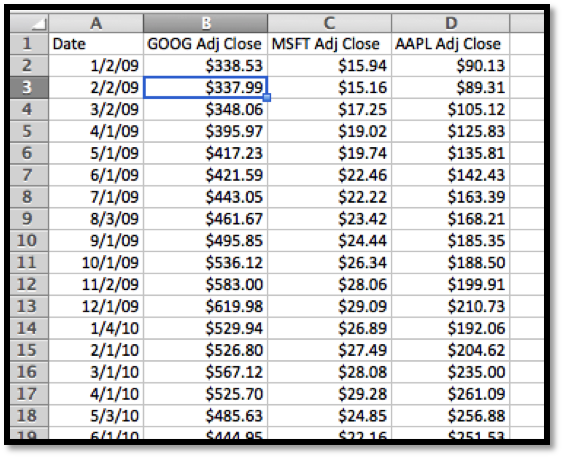
\includegraphics[width=0.8\linewidth]{images/sec1-3-9SharePrices.png}
\end{figure}
\par

Next we want to compute the number of shares for each stock.  This is 10 times the closing price of Google divided by the closing price of the stock we selected.
%
\leavevmode%
\begin{figure}
\centering
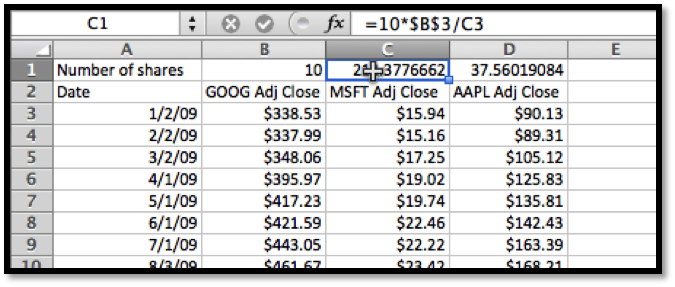
\includegraphics[width=0.8\linewidth]{images/sec1-3-10ShareAjustments.png}
\end{figure}
\par
In the formula for the number of shares of MSFT, we used \textdollar{}B\textdollar{}3 for the initial price of GOOG.  This is an absolute cell reference.  When we copy the formula from cell C1 to cell D1, the new formula is =10*\textdollar{}B\textdollar{}3/D3.  This formula in cell D1 asks for 10 times the value in cell B3, divided by the value in the 2 rows below the cell of the formula.  %
\begin{assemblage-untitled}\label{assemblage-8}
\terminology{Absolute references} refer to a particular column and/or row.  The dollar sign '\textdollar{}' is used to fix the reference.%
\par

\terminology{Relative references} refer to the cell the same distance away from the cell containing the formula.%
\end{assemblage-untitled}
\par

We continue our example by computing the change in value of our GOOG portfolio in the first month.  That will be the share price at the beginning of the next month minus the share price at the beginning of the month, times the number of shares.  For January 2009, for GOOG this becomes =(B4-B3)*B\textdollar{}1.%
\leavevmode%
\begin{figure}
\centering
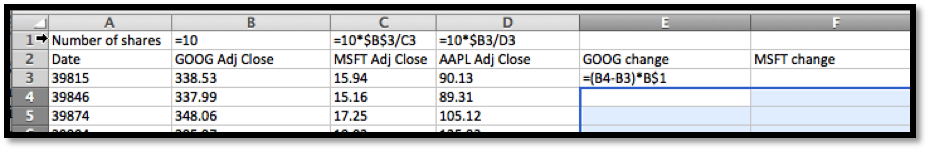
\includegraphics[width=0.9\linewidth]{images/sec1-3-11.png}
\end{figure}
\par
Since we have properly used relative and absolute references, we can now copy this formula to complete the chart, and Excel will modify the formula appropriately.%
\leavevmode%
\begin{figure}
\centering
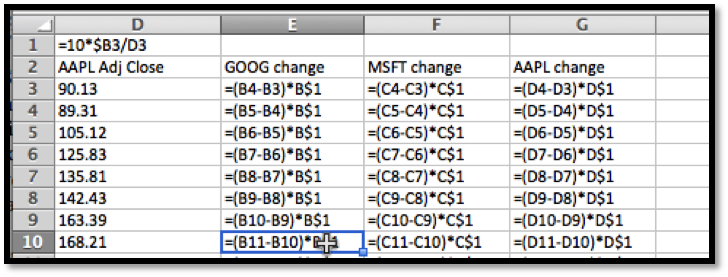
\includegraphics[width=0.8\linewidth]{images/sec1-3-12.png}
\end{figure}
\par
We note that the rows and columns can be independently made absolute or relative.  Thus if we are looking at a formula in cell A1, and see a reference to B2 it means the cell one below and to the right of the location of the formula.  If we see \textdollar{}B2 it means the cell in column B that is one row down from the formula.  If we see B\textdollar{}2 it means the cell in row two that is one column to the right of the formula.%
\par

When we concert back to see the values, we see that an original investment of \textdollar{}3,385.30 would have made a profit of \textdollar{}3,073.70 in GOOG stock, \textdollar{}2,128.02 in MSFT stock and \textdollar{}11,826.60 in AAPL stock.  Once again we use the SUM function and a cell range to add the values in the column.  We also use the split screen icons in the scroll bars to be able to see the correct rows and columns.%
\leavevmode%
\begin{figure}
\centering
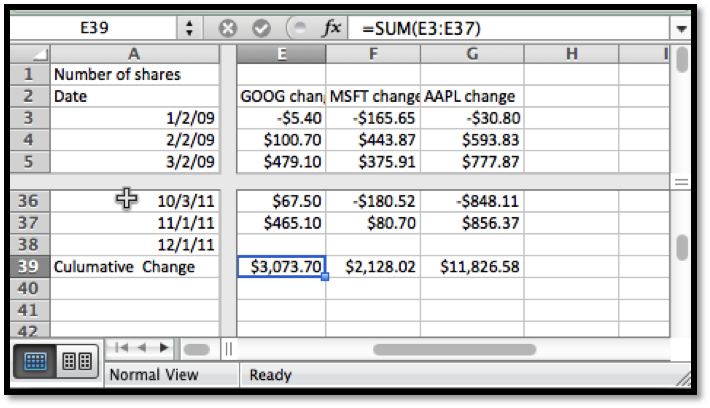
\includegraphics[width=0.8\linewidth]{images/sec1-3-13.png}
\end{figure}
\par
\terminology{Named Cell References}%
\par
An alternative to using absolute references in formulas is to name the cells. %
\begin{assemblage-untitled}\label{assemblage-9}
By default, Excel names each cell by its row and column.  We can use the name cell in the upper left corner of the Excel sheet to change the name from the letter/number format into a descriptive name.%
\end{assemblage-untitled}
\par

The more descriptive name can be useful when constructing and documenting the process we are using for our computations.  Consider the previous example with the rich uncle.  In cells B1, C1, and D1, we had the number of shares of Google, Microsoft, and Apple we could have had in the portfolio.  Better names for those cells would then be SharesGOOG, SharesMSFT, and SharesAAPL.  We can name a cell by editing the name box at the left side of the formula bar.%
\leavevmode%
\begin{figure}
\centering
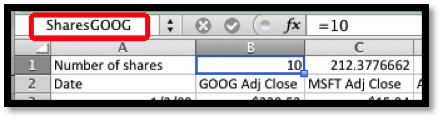
\includegraphics[width=0.4\linewidth]{images/sec1-3-14.png}
\end{figure}
\par
We can then use the names in formulas.  In general, the formulas with nicely named variables are easier to read.
%
\leavevmode%
\begin{figure}
\centering
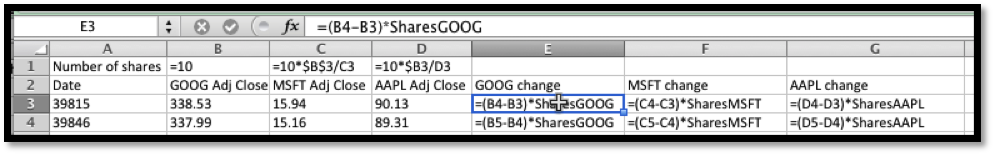
\includegraphics[width=0.8\linewidth]{images/sec1-3-15.png}
\end{figure}
\par
\terminology{
Getting Help
}%
\par
One of the ways that doing mathematics with a program like Excel differs from working with a calculator is that computer programs have help features.  It is worthwhile pointing out two that come with Excel.  We illustrate both with the SUM function we have used a number of times.%
\par

When we call Help from the top menu, we are given a pop up window for Excel Help.  It has a number of topics listed by default.  It also has a bar for searching topics.%
\leavevmode%
\begin{figure}
\centering
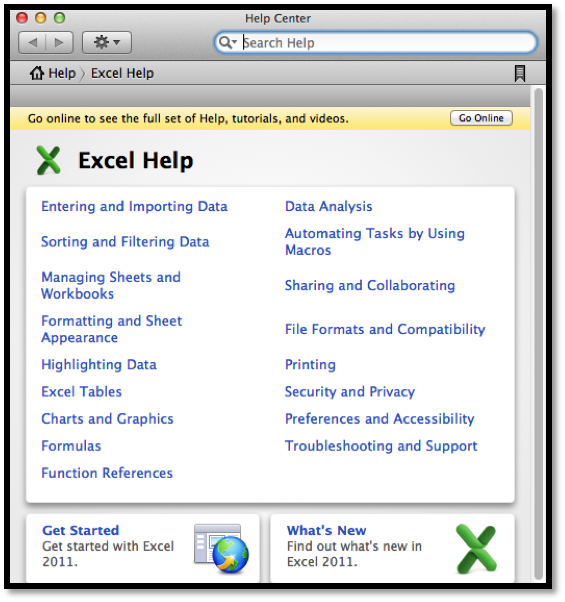
\includegraphics[width=0.8\linewidth]{images/sec1-3-16.png}
\end{figure}
\par
We type the name of the command we are looking for and we are given a page of help for that command.%
\leavevmode%
\begin{figure}
\centering
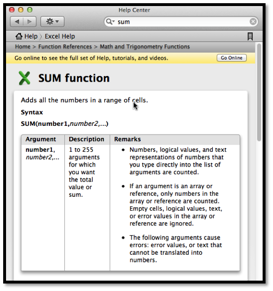
\includegraphics[width=0.8\linewidth]{images/sec1-3-17.png}
\end{figure}
\par

A second kind of help is the formula builder from the formula ribbon.  It gives a more concise help when you do not remember the exact syntax of a command.%
\leavevmode%
\begin{figure}
\centering
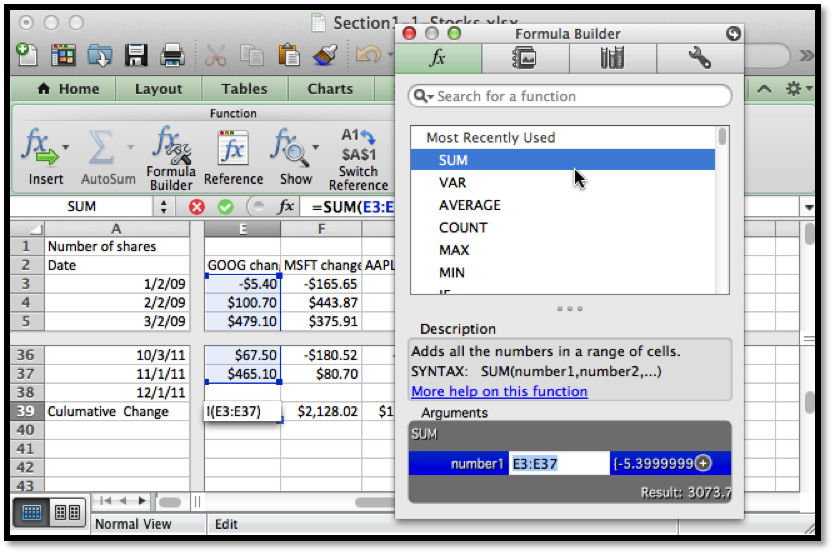
\includegraphics[width=0.8\linewidth]{images/sec1-3-18.png}
\end{figure}
\par
A third source of help is simply to do a web search for excel help.  To find how to do a computation with an exponential functions you can search for “Excel formulas exponential.”%
\par
\terminology{
Other Details}%
\par
Excel is a rich and complex tool.  We will be looking at more features as we go through the course.  There are several that are worth pointing out explicitly at this point.%
\leavevmode%
\begin{itemize}[label=\textbullet]
\item{}For ordinary arithmetic, Excel uses the standard symbols of +, -, *, /, and \textasciicircum{} for plus, minus, times, divided by, and raising to a power.
%
\item{}We can also use the SUM, PRODUCT, QUOTIENT, and POWER commands for ordinary arithmetic.
%
\item{}The order of operations used by Excel differs from the traditional order of operations when it comes to taking powers of negative numbers.  The problem is illustrated in evaluating  \(-3^2\), which has a negative sign and an exponentiation. In all math classes you have taken this is interpreted as \(-(3^2)\) or \(-9\), with exponentiation done first.  In Excel, this is interpreted as \((-3)^2\) or 9, with negation done first.  When in doubt, use parenthesis to make the order of operations explicit.
%
\item{}Excel also has the other mathematical functions you have used before.  The functions for square root, log base 10, log base e, and e to the power of, are respectively, SQRT, LOG, LN, and EXP.
%
\item{}The value of e is represented by EXP(1). 
%
\item{}Excel has a number of very useful operations on collections of numbers.  We start with easy ones where the name is self explanatory, like SUM, AVERAGE, COUNT, MIN, and MAX.
%
\end{itemize}
\typeout{************************************************}
\typeout{Exercises 1.3.1 Exercises 1.3 Introduction to Excel Spreadsheets}
\typeout{************************************************}
\subsection[{Exercises 1.3 Introduction to Excel Spreadsheets}]{Exercises 1.3 Introduction to Excel Spreadsheets}\label{exercises-set-sec-1-3}
\begin{exerciselist}
\item[1.]\hypertarget{exercise-42}{}  Produce a spreadsheet where the first 100 rows are used.  The cell in row n and column A should have value n.  The cell in row n and column B should have value 2*n.  You should be able to do this by typing in the value of 4 cells and using quick fill.
%
\par\smallskip
\item[2.]\hypertarget{exercise-43}{}  Produce a spreadsheet where the first 100 rows are used.  Column A should contain the first 100 odd numbers.  Column B should contain multiples of 7 starting with 21.
%
\par\smallskip
\item[3.]\hypertarget{exercise-44}{}  Start with the worksheet given.  Complete the worksheet in such a way that if the values of x, y, and z are changed, the other values are automatically recomputed.
%
\par\smallskip
\leavevmode%
\begin{figure}
\centering
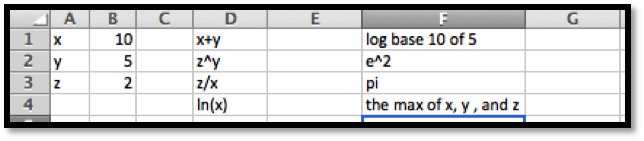
\includegraphics[width=0.7\linewidth]{images/sec1-3-e1.png}
\end{figure}
\item[4.]\hypertarget{exercise-45}{}  Produce a spreadsheet where the first 101 rows are used.  Row 1 should be used for labels. Column A should contain integers from 1 to 100.  Columns B through F should contain the squares, cubes, square roots, logs base 10 and natural logs of the entries in columns A.
%
\par\smallskip
\item[5.]\hypertarget{exercise-46}{}  Start with the spreadsheet section below.
\leavevmode%
\begin{figure}
\centering
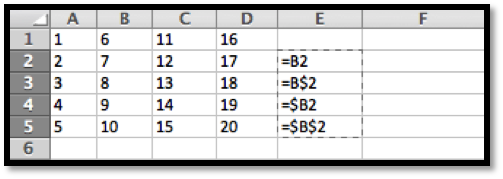
\includegraphics[width=0.6\linewidth]{images/sec1-3-e2.png}
\end{figure}
 
 
	If column E is copied and pasted into column G, give both the formula and value for each non-empty cell in column G.
%
\par\smallskip
\item[6.]\hypertarget{exercise-47}{}  We would like to really understand what happens when we use quick fill. %
\leavevmode%
\begin{enumerate}[label=(\Alph*)]
\item\hypertarget{li-66}{}
 Let's consider the entries =A1, =\textdollar{}A1, =A\textdollar{}1, and =\textdollar{}A\textdollar{}1 in row 2.  Do quick fill below to fill in 3 more rows and see what happens. Clearly in the first row these cells all now point to cell A1 and the value returned is 1. After the first row we get a mixture of values. Why?%
\leavevmode%
\begin{figure}
\centering
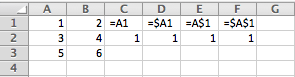
\includegraphics[width=0.8\linewidth]{images/sec1-3-e3.png}
\end{figure}
\item\hypertarget{li-67}{}
 Next, we can set up the values in column D. Do quick fill to fill in the 3 columns to the right? Explain the pattern of values we see.
 \leavevmode%
\begin{figure}
\centering
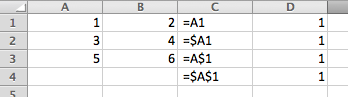
\includegraphics[width=0.8\linewidth]{images/sec1-3-e4.png}
\end{figure}
 
%
\end{enumerate}
\par\smallskip
\item[7.]\hypertarget{exercise-48}{}  Complete the spreadsheet section below so that columns A through C are complete for numbers 1 to 100.  (The value for a should be a random number generated by the formula in cell E1.)
%
\par\smallskip
\leavevmode%
\begin{figure}
\centering
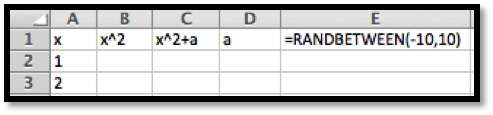
\includegraphics[width=0.6\linewidth]{images/sec1-3-e5.png}
\end{figure}
\item[8.]\hypertarget{exercise-49}{}  Using the help functions to check syntax, write a formula for cell B2, that looks at the value for cell A2, and if it is negative, returns the square of it, and if positive returns its square root.
%
\par\smallskip
\item[9.]\hypertarget{exercise-50}{} Using your favorite source on the web create a spreadsheet that has the closing price of your favorite stock on the first day of the month for the past 5 years.  Compute the change in adjusted stock price for each month and identify which month had the greatest increase.  
(\href{http://finance.yahoo.com/}{http://finance.yahoo.com/}) is one source for such data.)
%
\par\smallskip
\item[10.]\hypertarget{exercise-51}{} Using your favorite source on the web create a spreadsheet that has the closing price of your favorite stock on the first day of the month for the past 5 years.  Compute the percentage change in adjusted stock price for each month and identify which month had the greatest increase.  
%
\par\smallskip
\item[11.]\hypertarget{exercise-52}{} Create a spreadsheet showing the Consumer Price Index by month from 1930-2010.  (Good sources are 
\href{http://inflationdata.com/}{http://inflationdata.com/} 
 and \href{http://www.bls.gov/cpi/}{http://www.bls.gov/cpi/} at the Bureau of Labor Statistics.)  Compute the percentage change between January and July for each year.  Which year had the greatest percentage change in the first half of the year?
%
\par\smallskip
\end{exerciselist}
\typeout{************************************************}
\typeout{Section 1.4 Graphing functions with Excel}
\typeout{************************************************}
\section[{Graphing functions with Excel}]{Graphing functions with Excel}\label{sec-1-4-GraphingFunctionsExcel}

One area where Excel is different from a graphing calculator is in producing the graph of a function that has been defined by a formula.  It is not difficult, but it is not as straight forward as with a calculator. It is a skill worth developing however.  When we are given a formula as part of a problem, we will want to easily see a graph of the function. %
\par

We will walk through the process for producing graphs for three examples of increasing complexity.  For the first example we have a specific function and specific range in mind, say \(y=x^2-6 x\) over \(-10 \le x \le 10\).  For the second example, we would like to use parameters in the formula, for example, \(y = a x^2 + b x + c\), with specified values of a, b, and c, and have the ability to easily change the values of the parameters and see the graph.  For the third example we would also like to have the ability to change the domain, graphing over \(xLow \le x \le xHigh\), where \(xLow\) and \(xHigh\) can easily be changed.%
\begin{example}[A basic graph]\label{example-5}
 graphing \(y=x^2-6 x\) over \(-10 \le x \le 10\).%
\leavevmode%
\begin{figure}
\centering
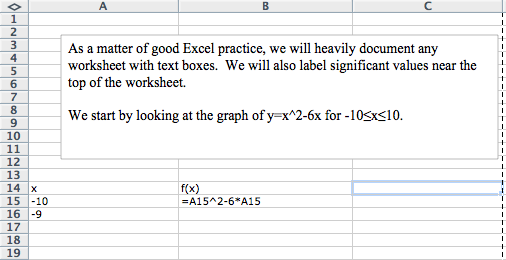
\includegraphics[width=0.8\linewidth]{images/sec1-4-1.png}
\end{figure}
\par

We start by producing a column for x and one for f(x).  In the column for x we start with values -10 and -9, so that we can complete the column with a quick fill.  Similarly, we start the f(x) columns in the first cell with the "x" replaced by the appropriate cell reference.  In this case the formula for f(x) is in cell B15 and x is in cell A15.%
\par

We then use quick fill and quick copy to fill out the table.%
\leavevmode%
\begin{figure}
\centering
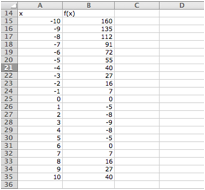
\includegraphics[width=0.6\linewidth]{images/sec1-4-2.png}
\end{figure}
\par

With the values of the cells filled in we highlight the cells we want to graph (A14 through B35) and add a scatter plot for the highlighted values.
%
\leavevmode%
\begin{figure}
\centering
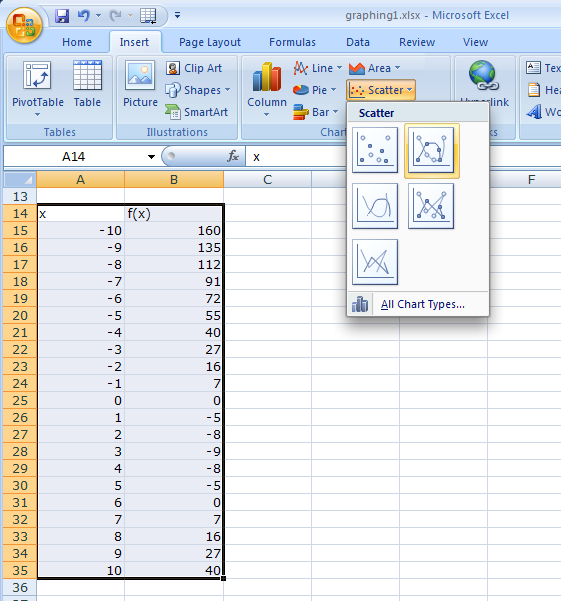
\includegraphics[width=0.8\linewidth]{images/sec1-4-3.png}
\end{figure}
\par

(The location of the scatterplot will be a bit different with Macs.  The scatterplot is in the Charts ribbon, under other, on Macs.)  This gives the desired graph.%
\leavevmode%
\begin{figure}
\centering
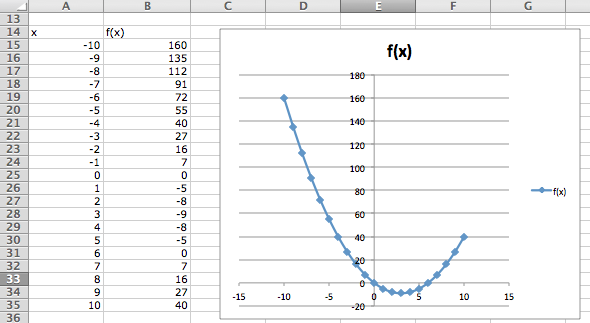
\includegraphics[width=0.8\linewidth]{images/sec1-4-4.png}
\end{figure}
\end{example}
\begin{example}[A graph with parameters]\label{example-6}
 – graphing \(y=x^2-6 x\) as an example of 
\(y = a x^2 + b x + c\) over the domain \(-10 \le x \le 10\).%
\par
For the second example, we want the same graph, but we want the ability to easily convert the graph of our first quadratic into a different quadratic function.  The solution is to consider a, b, and c to be parameters that we can change.%
\par
Toward the top of the worksheet, we put the labels \(a\), \(b\), and \(c\), and give values for those parameters.  In this case the values of \(a\), \(b\), and \(c\) are in cells B9, B10, and B11 respectively.%
\par
Now we set up the problem in the same way we did above except that we are using absolute references for \(a\), \(b\), and \(c\), and relative references for \(x\).
%
\leavevmode%
\begin{figure}
\centering
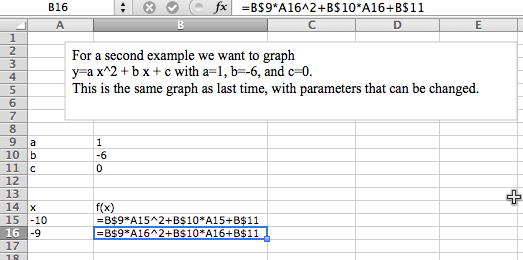
\includegraphics[width=0.8\linewidth]{images/sec1-4-5.png}
\end{figure}
\par
Now, we once again do a quick fill to complete the table, and then add a scatterplot.%
\leavevmode%
\begin{figure}
\centering
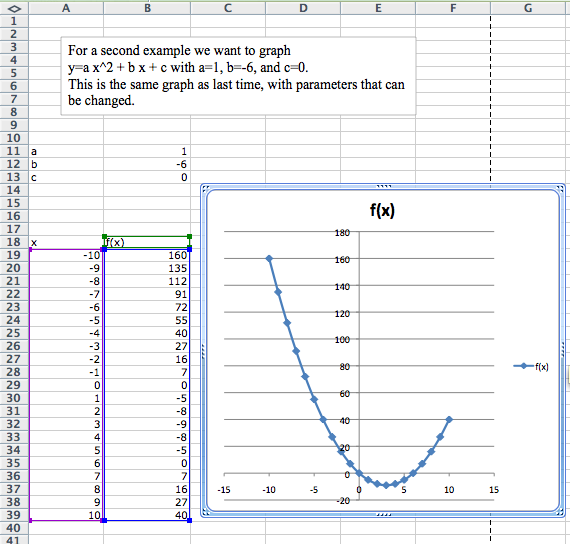
\includegraphics[width=0.8\linewidth]{images/sec1-4-6.png}
\end{figure}
\par
The difference with this second example is that if I now want to look at the graph of \(y = -x^2 + 3 x + 10\), I simply change the values of the parameters \(a\), \(b\), and \(c\).%
\leavevmode%
\begin{figure}
\centering
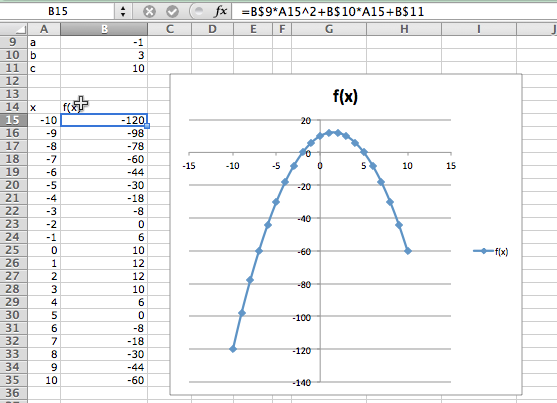
\includegraphics[width=0.8\linewidth]{images/sec1-4-7.png}
\end{figure}
\end{example}
\begin{example}[Controlling the viewing window]\label{example-7}
 graphing \(y=x^2 - 6 x\) as an example of \(y = a x^2 + b x + c\) over the domain \(-10 \le x \le 10\), but with the ability to easily chance the domain of the graph.%
\par
Often, when we graph, we will want to change the domain of the graph.  Most easily, I may want to zoom in on a particular region to get a better view of some interesting feature.  I may want to look closely at several different regions.%
\par
To do this we will again plot 21 points, but we want to have control of the starting point and the change in x between the first and second points.  First we add labels and values for x-start and x-step.  Then we need a bit of care in defining the values of x.  The first value of x (cell A18) is the value of x-start.  Every other value of x is defined as the previous value of x plus the value of x-step.%
\leavevmode%
\begin{figure}
\centering
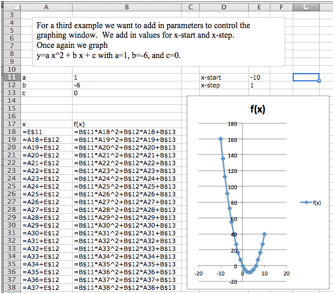
\includegraphics[width=0.8\linewidth]{images/sec1-4-8.png}
\end{figure}
\par
In this case I want a better look at the vertex of the parabola.  I decide I want to see the graph for \(0 \le x \le 5\).  My value for x-start is 0.  My value for x-step is one twentieth of the distance from 0 to 5, or \((5-0)/20 = 0.25\).  I plug those values in and see the graph.%
\leavevmode%
\begin{figure}
\centering
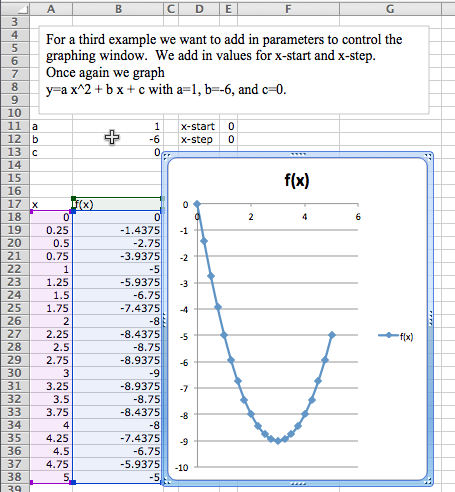
\includegraphics[width=0.8\linewidth]{images/sec1-4-9.png}
\end{figure}
\end{example}
\par
\terminology{Graphing more than one function}%
\par
We would also like to put two or more graphs together.  For our examples, we will want to use the functions \(f(x) = x – 3\), \(g(x) = (x^2 – x)/10\), and \(h(x) = x^3 – x\).  We start by using the procedure given above to make a chart of values for the three functions.%
\leavevmode%
\begin{figure}
\centering
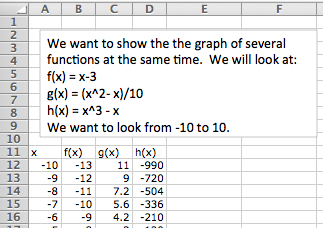
\includegraphics[width=0.6\linewidth]{images/sec1-4-10.png}
\end{figure}
\par
We then simply select the cells for \(x\) and the functions we want graphed together and produce a scatterplot as before.  (To graph \(g(x)\) and \(h(x)\) together, we want to select the columns for \(x\), \(g(x)\), and \(h(x)\).)%
\leavevmode%
\begin{figure}
\centering
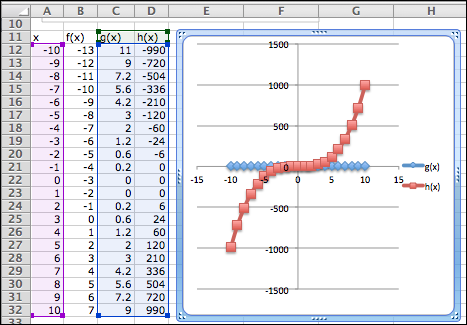
\includegraphics[width=0.8\linewidth]{images/sec1-4-11.png}
\end{figure}
\par
On problem with the graph of \(g(x)\) and \(h(x)\) together is that the functions have different orders of magnitude, so we do not see that \(y = g(x)\) is a parabola.  One remedy is to use a secondary axis for the graph of \(h(x)\).  (Simply double click on one of the points for \(h(x)\), and select secondary axis from the axes tab.)%
\par
\terminology{Formatting a chart}%
\par

Excel has a lot of ways to add formatting to a graph or chart, many more than we want to be concerned with at this point.  We simply point out a few and leave it to the reader to explore how this should be used for a good visual presentation.  If you click once on the chart to select it, the Chart tab in the home ribbon, adds sub-tabs for layout and format.  With Chart Title, you can add a title to the chart, then edit it.  The Axes icon allows you to add titles for the axes.  If you select a data point form \(g(x)\), you can then use the Data Labels icon to add values next to the points.  The chart with these annotations is given below.  The rule of thumb to follow is to add enough annotations for a reader to be able to easily understand what is happening in the chart.%
\leavevmode%
\begin{figure}
\centering
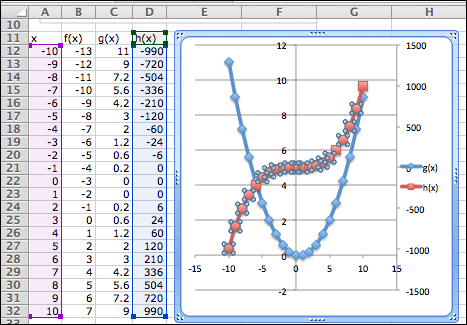
\includegraphics[width=0.8\linewidth]{images/sec1-4-12.png}
\end{figure}
\par
It is also worthwhile to note that you can manually set the y-range of a graph by double clicking on the axis and setting the values.  This is particularly useful of the function has a vertical asymptote.%
\par
\terminology{Online graphing tools: Wolfram Alpha}%
\par
Throughout this book, we are limiting ourselves to mathematical tools that the student can reasonably expect to find in a generic work environment.  That is one of the reasons for focusing on using spreadsheets and Excel.  A second reason is that we will spend a significant amount of time on functions defined by data points, where we then try to construct a formula.  However when we are starting with a formula, there are easier ways to produce a graph.  The simplest is to use the free website, Wolfram Alpha.  For example to obtain a graph of the functions \(f(x) = x^2 – 3 x\), as \(x\) ranges from \(-5\) to \(5\), we simply type “plot x\textasciicircum{}2 – 3 x for x from -5 to 5” and obtain:%
\leavevmode%
\begin{figure}
\centering
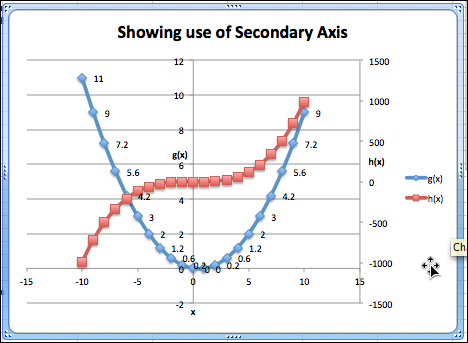
\includegraphics[width=0.8\linewidth]{images/sec1-4-13.png}
\end{figure}
\par
We will return to Wolfram Alpha from time to time, when we have nice formulas to manipulate. %
\typeout{************************************************}
\typeout{Exercises 1.4.1 Exercises 1.4 Graphing functions with Excel}
\typeout{************************************************}
\subsection[{Exercises 1.4 Graphing functions with Excel}]{Exercises 1.4 Graphing functions with Excel}\label{exercises-set-sec-1-4}
\begin{exerciselist}
\item[1.]\hypertarget{exercise-53}{} Produce a worksheet that with a graph of the function \(f(x) = x^2 - 5 x\), with \(x\) going from -10 to 10 by 1.
%
\par\smallskip
\item[2.]\hypertarget{exercise-54}{} Produce a worksheet that with a graph of the function 
\(g(x) = (x^2 - 5 x)/(x^2 + 7 x + 10)\), with \(x\) going from -10 to 10 by 1.  Explain why the graph is inaccurate.  (Pay attention to places where there should be asymptotes.)%
\par
2* - Extra credit) – Fix the graph from problem 2 by adjusting the set of x-values used.
%
\par\smallskip
\item[3.]\hypertarget{exercise-55}{} Produce a worksheet with a graph of \(h(x) = x^3 + a x^2 + b x + c\) for \(x\) from -10 to 10, where the values of \(a\), \(b\), and \(c\) can be changed and the graph will update automatically.  For initial values, use \(a = -2\), \(b = 1\), and \(c = -11\).
%
\par\smallskip
\item[4.]\hypertarget{exercise-56}{} Produce a worksheet with a graph of \(k(x) = (x^2 + a x + b)/( x + c)\) for x from -10 to 10, where the values of \(a\), \(b\), and \(c\) can be changed and the graph will update automatically.  For initial values, use \(a = -5\), \(b = 2\), and \(c = -11\).
%
\par\smallskip
\item[5.]\hypertarget{exercise-57}{} Produce a worksheet with a graph of \(h(x) = x^3 -2 x^2 +  x -11\) for \(x\) going from a to b, where the values of \(a\) and \(b\) can be changed and the graph will update automatically.  For initial values, use \(a = -5\) and \(b = 5\).
%
\par\smallskip
\item[6.]\hypertarget{exercise-58}{} Produce a worksheet with a graph of \(k(x) = (x^2 -5 x + 2)/( x -11)\) for \(x\) going from \(a\) to \(b\), where the values of a and b can be changed and the graph will update automatically.  For initial values, use \(a = -5\) and \(b = 5\).
%
\par\smallskip
\item[7.]\hypertarget{exercise-59}{} (Writing assignment) Write a report of 2 pages or less on the graph of the function
\(f(x) = (x^2 + 7 x + 10)/(x^2 - 3 x +2)\).  The report should be in Word (or other word processor) format with at least 2 graphs that illustrate different features by looking at different viewing windows.
%
\par\smallskip
\item[8.]\hypertarget{exercise-60}{} Produce a worksheet with graphs of \(f(x) = 2 x + 5\) and \(g(x) = x^3 – 9 x\), for x going from -10 to 10.  Use secondary axes so that both graphs use the full plotting window.
%
\par\smallskip
\item[9.]\hypertarget{exercise-61}{} Produce a worksheet with graphs of \(h(x) = (x^3 – 9 x)/(x^2 + 3 x + 35/16)\) and \(k(x) = 2 x^2 + 5\), for x going from -10 to 10.  Use secondary axes so that both graphs use the full plotting window.  Adjust the range of \(y\) values used to make the graph reasonable.
%
\par\smallskip
\item[10.]\hypertarget{exercise-62}{} Produce a worksheet with graphs of \(f(x) = 2 x + 3\) and \(g(x) = -2 x +5\), for \(x\) going from -10 to 10.  Add a title to the chart.  Do something interesting with the fonts or other options and explain what you did.
%
\par\smallskip
\item[11.]\hypertarget{exercise-63}{} Use Wolfram Alpha to produce a graph of \(f(x) = x^3 - 16 x\), for \(x\) going from -5 to 5.  Use your favorite screen capture software and paste the result into an Excel worksheet.
%
\par\smallskip
\end{exerciselist}
\typeout{************************************************}
\typeout{Section 1.5 Using Excel to find best-fit curves}
\typeout{************************************************}
\section[{Using Excel to find best-fit curves}]{Using Excel to find best-fit curves}\label{sec-1-5-IntroBestFitCurves}
\terminology{Overview}%
\par
In the sections 1.1 and 1.2 we looked at useful mathematical models and formulas that we anticipate seeing repeatedly in the business environment.  If we are given equations that model the processes we are interested in, then this approach works. What happens though if we are not given equations? Many important functions in business are quite often defined by data.  Examples include past sales, material costs, and consumer demand. %
\par
If we are given a data set, we can find a best fitting curve.  A straightforward approach is to assume that the data represents the output of a nice formula. In real life applications we will often see that so-called noise can complicate the situation.  (For example, if I am looking at sales at a fast food restaurant, our model will have noise from traffic jams and bad weather outside.) For the purpose of this course we will assume that the data will be reasonably nice, although some noise may be evident. The problem of producing a best fitting curve to data can be broken into two pieces: %
\leavevmode%
\begin{enumerate}
\item\hypertarget{li-68}{}We need to decide what kind of curve, or what model we want to use. %
\item\hypertarget{li-69}{}We want to be able to set the parameters (the constants) in the model to give the best fit.%
\end{enumerate}
\par
Coming up with a theoretical reason why we want to use a particular model in a given case forms the content of a large number of your business courses, both courses you have already taken and courses you are yet to take.  The models that come up repeatedly in the theoretical courses are given names and used without redoing the theoretical foundation for the model.  (This is why we introduced the normal distribution and the logistic growth function, neither of which looks like a simple equation.)  In this course, we will be happy with simple heuristic arguments on which model to choose.
%
\par
The second half of the problem is deciding how to choose the parameters to give the curve that does the best job of fitting the data.  A moment of reflection shows deciding on the correct definition of “best fitting” is a nontrivial task beyond the scope of this course.  For the time being we will accept the standard definition 
%
\begin{assemblage-untitled}\label{assemblage-10}
The \terminology{best fitting curve} minimizes the sum of the squares of the differences between the measured and predicted values. 
%
\end{assemblage-untitled}
\par
We will come back to that definition later in the course, when we know more calculus, but for now we simply note that it is the standard definition, and is used by Excel.  Instead, we will focus on using Excel to produce a best fitting curve of the appropriate model. Excel has a preprogrammed feature that will find the best fitting equation for a data set for a select number of functions:%
\leavevmode%
\begin{itemize}[label=\textbullet]
\item{}Linear model%
\item{}Exponential model%
\item{}Polynomial model%
\item{}Logarithmic model%
\item{}Power model%
\end{itemize}
\par
We will show how to find an equation for a data set, assuming we know what model would be the best one to represent the data.

%
\par
\terminology{Best fitting linear curves}

%
\par
For a first example, we are running a widget factory and have the following data on employee performance:

  \leavevmode%
\begin{figure}
\centering
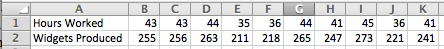
\includegraphics[width=0.8\linewidth]{images/sec1-5-1.png}
\end{figure}
 

%
\par
(A parenthetical note:  In economics, widget is a placeholder name for a generic manufactured device.  It is only in recent times that it has also become a small computer GUI unit.)
%
\par
We would like a formula for widgets produced as a function of hours worked.  Since we can see two entries each, for 36, 43, and 44 hours worked, there cannot be a function that hits all our data exactly.  While we expect a linear function, we are not surprised if there is random noise, as a worker may take a break, or be particularly focused on a given day.  We start by creating a scatterplot for my data.

  \leavevmode%
\begin{figure}
\centering
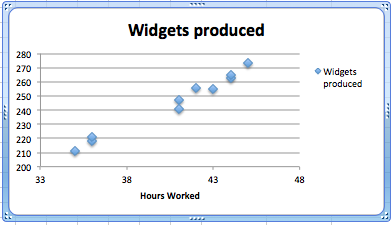
\includegraphics[width=0.8\linewidth]{images/sec1-5-2.png}
\end{figure}
 

%
\par
We right click (control-click on a mac) on one of the data points and we get a contextual menu.  We select \terminology{Add Trendline}.

  \leavevmode%
\begin{figure}
\centering
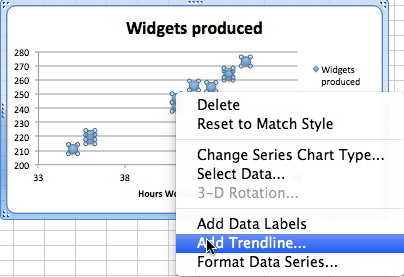
\includegraphics[width=0.8\linewidth]{images/sec1-5-3.png}
\end{figure}
 

%
\par
When adding a trend line, we need to select from a number of options.  The first option concerns the mathematical model we want to choose.  Given that we suspect the number of widget produced will be roughly proportional to the hours worked, we want to use a linear model, so we make that choice.  Under options, we want to display the equation on the chart.

  \leavevmode%
\begin{figure}
\centering
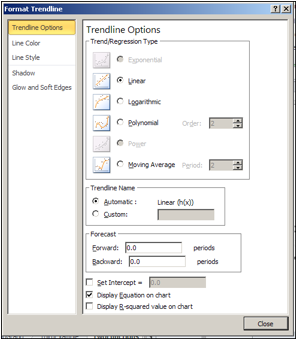
\includegraphics[width=0.8\linewidth]{images/sec1-5-4.png}
\end{figure}
 

%
\par
We have added a linear trend line to the graph and can also see the equation for the line.  We could use that equation to plan how many hours we want our workers on the job based on the number of widgets we expect to sell.

  \leavevmode%
\begin{figure}
\centering
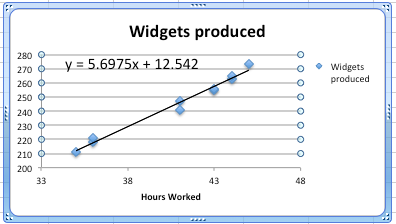
\includegraphics[width=0.8\linewidth]{images/sec1-5-5.png}
\end{figure}
 

%
\par
Having found a best fitting line, I want to copy the equation back into my spreadsheet and to be able to compare the values in my data with the projections from my equation.  You should notice that the equation Excel produces in the chart is written in standard mathematical notation, while the corresponding equation in cell B3 is in Excel notation.  (In Excel notation we need a symbol for multiplication rather than simply putting a number and variable together.  In Excel notation, we also use a cell reference, B1, rather than a variable, x.)

  \leavevmode%
\begin{figure}
\centering
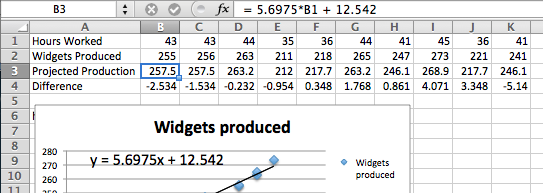
\includegraphics[width=0.8\linewidth]{images/sec1-5-6.png}
\end{figure}
 

%
\par
\terminology{Checking and improving our equations}
%
\par
 When finding the best fitting curve to data we have gathered, we need to pay attention to the model we have chosen and to the range to which we want to apply it.  In our example, the linear fit looks pretty good.  However we should be careful about using it on too wide a domain.  According to our model, a worker who works no hours produces 12.52 widgets a week, which is obviously silly.  In the other direction it predicts that a worker who worked 168 (= 7 x 24) hours a week would produce almost 970 widgets, instead of predicting a collapse from exhaustion.
%
\par
The other issue is the choice of a model.  We chose a linear model.  An argument could easily be made for a proportional model.  (A worker who works no hours produces no widgets.)  We can switch to the proportional model by setting the y-intercept to 0 in options for the trend line.  Then the equation is  
\begin{equation*}(Widgets Produced) = 6.00026*(Hour Worked)\end{equation*}
instead of our original equation of 
\begin{equation*}(Widgets Produced) = 5.6975*(Hours Worked)+12.54.\end{equation*}

  \leavevmode%
\begin{figure}
\centering
\includegraphics[width=0.8\linewidth]{images/sec1-5-7.png}
\end{figure}
 

%
\par
We should also be careful about trying to get a better fit by using an inappropriate model.  In our case, we can get a better fit by allowing the curve to be a 6th degree polynomial.  However the resulting equation does not make sense.  It predicts that a worker will produce about quarter million widgets with a 1-hour work week, and -1500 widgets with a 55-hour work week.

  \leavevmode%
\begin{figure}
\centering
\includegraphics[width=0.8\linewidth]{images/sec1-5-8.png}
\end{figure}
 

%
\par
\terminology{Fitting the Consumer Price Index (CPI) to a best fitting curve;} an extended example

%
\par
For our second example, we will look at the consumer price index and try and fit it to a model.  This example will illustrate several issues we need to keep in mind when building models.  We obtained data for the consumer price index from \href{http://inflationdata.com/inflation/Consumer_Price_Index.HistoricalCPI.aspx}{http://inflationdata.com/inflation/Consumer\textunderscore{}Price\textunderscore{}Index.HistoricalCPI.aspx}.  

%
\par
The data from 1960 to 2011 is in the worksheet Section1-4Example.xlsx.

  \leavevmode%
\begin{figure}
\centering
\includegraphics[width=0.8\linewidth]{images/sec1-5-9.png}
\end{figure}
 

%
\par
Since we expect prices to rise as a percentage of the current prices, we expect the CPI to be modeled by an exponential curve.  We start by selecting the data, producing a scatterplot, and adding a best fitting curve using an exponential model.  We will always select the option to show the equation on the chart.

  \leavevmode%
\begin{figure}
\centering
\includegraphics[width=0.8\linewidth]{images/sec1-5-10.png}
\end{figure}
 

%
\par
This first attempt gives an exponential formula, but it is unsatisfactory for a number of reasons.%
\leavevmode%
\begin{itemize}[label=\textbullet]
\item{}That constant only shows one significant digit, which is not enough to make meaningful predictions.%
\item{}The font size is too small to easily read off the resulting equations.%
\item{}The constant coefficient is ridiculously small because it gives the projected value of the index in the year 0. Another way of thinking about this is that the values we are evaluating this exponential function at run in the thousands!.%
\item{}The graph does not look like a very good fit.  The plot of the numbers actually looks as though it represents three different graphs.%
\end{itemize}
\par
We will work through the problems one at a time.

%
\par
The first problem is that the equation Excel has given us does not have enough significant digits to make useful predictions.  We want to right click on the equation, select “Format Trendline Label”.  We are given a dialog box that lets us make formatting options.  Since the lead coefficient is so small, we want the numbers formatted in Scientific notation.  We choose 4 digits beyond the decimal point in that notation.  

  \leavevmode%
\begin{figure}
\centering
\includegraphics[width=0.8\linewidth]{images/sec1-5-11.png}
\end{figure}
 

%
\par
This gives us a better equation.  It should be noted that our pictures in this book use the font option in the formatting to use a larger sized font.

  \leavevmode%
\begin{figure}
\centering
\includegraphics[width=0.8\linewidth]{images/sec1-5-12.png}
\end{figure}
 

%
\par
The next issue to deal with is adjusting the year.  Looking at the raw data, the CPI was 100 sometime in 1983.  Thus we simply add an extra column to our spreadsheet where the adjusted year is the current year minus 1983.  In our graph, we also adjust the labels so a reader can still understand our chart.

  \leavevmode%
\begin{figure}
\centering
\includegraphics[width=0.8\linewidth]{images/sec1-5-13.png}
\end{figure}
 

%
\par
Now we want to look at the more serious question, the one that says the model does not fit very well.  Looking at our data, the inflation rate seems to fall into roughly 3 blocks, the years before 1973, the years from 1973-1983, and the years after 1983.  We would want to go back to our economics classes and find an argument that says this division of years is reasonable.  Using the same menu that lets us add a trend line, we can edit the source data.  We want to restrict to the years after 1983.  In our case, that means restricting to rows 1 to 30.

  \leavevmode%
\begin{figure}
\centering
\includegraphics[width=0.8\linewidth]{images/sec1-5-14.png}
\end{figure}
 

%
\par
This breaks the data into two pieces.  The first piece is the period from 1982 till 2011.  As we see, the exponential model fits quite well in that case.
 
  \leavevmode%
\begin{figure}
\centering
\includegraphics[width=0.8\linewidth]{images/sec1-5-15.png}
\end{figure}
 

%
\par
The second piece is the period from 1973 till 1983.  Once again, the exponential model fits quite well over that period.  Notice that the exponent is quite different in the two periods.%
\leavevmode%
\begin{figure}
\centering
\includegraphics[width=0.8\linewidth]{images/sec1-5-16.png}
\end{figure}
\par
The obvious questions that arrises is to figure out what happened in 1983 that caused the economic model to shift.  That questions is beyond the scope of this course.%
\typeout{************************************************}
\typeout{Exercises 1.5.1 Exercises: Using Excel to find best fit curves}
\typeout{************************************************}
\subsection[{Exercises: Using Excel to find best fit curves}]{Exercises: Using Excel to find best fit curves}\label{exercises-set-sec-1-5}
\begin{exerciselist}
\item[1.]\hypertarget{exercise-64}{}  We have the following data on widget production:
%
\leavevmode%
\begin{table}
\centering
\begin{tabular}{cccccc}\hrulethick
Month&Jan&Feb&Mar&Apr&May\tabularnewline\hrulethin
Production&16,579&30,687&48,441&55,751&79,606\tabularnewline\hrulemedium
\end{tabular}
\end{table}
\leavevmode%
\begin{enumerate}[label=(\alph*)]
\item\hypertarget{li-79}{} Find the best fitting linear function for the data.%
\item\hypertarget{li-80}{} Give the production value that function predicts for May.%
\item\hypertarget{li-81}{} Give the production value that function predicts for July.%
\end{enumerate}
\par\smallskip
\item[2.]\hypertarget{exercise-65}{}  We have the following data on gizmo sales:
%
\leavevmode%
\begin{table}
\centering
\begin{tabular}{cccccc}\hrulethick
Month&Jan&Mar&Apr&July&Aug\tabularnewline\hrulethin
Units sold&1.505&9,042&13,018&21,873&22,636\tabularnewline\hrulemedium
\end{tabular}
\end{table}
\leavevmode%
\begin{enumerate}[label=(\alph*)]
\item\hypertarget{li-82}{} Find the best fitting linear function for the data.%
\item\hypertarget{li-83}{} Extend the chart to give the projected sales for each month from January through September.  (You need to add a row for predicted sales, and also add a number of columns for missing months.)%
\end{enumerate}
\par\smallskip
\item[3.]\hypertarget{exercise-66}{}  We have the following data on gadget revenue:
%
\leavevmode%
\begin{table}
\centering
\begin{tabular}{cccccc}\hrulethick
Units sold&3,000&5,000&7,000&9,000&11,000\tabularnewline\hrulethin
Revenue&16,161&24,783&34,484&38,014&33,030\tabularnewline\hrulemedium
\end{tabular}
\end{table}
\leavevmode%
\begin{enumerate}[label=(\alph*)]
\item\hypertarget{li-84}{} Find the best fitting linear function for the data.%
\item\hypertarget{li-85}{} Find the best fitting quadratic function for the data.%
\item\hypertarget{li-86}{} The data fits a quadratic function better than a linear function.  With a quadratic model we do not maximize revenue by selling as many units as possible.  Explain why this is reasonable in the real world.%
\item\hypertarget{li-87}{} Project the revenue for selling 15,000 units with both linear and quadratic models.%
\end{enumerate}
\par\smallskip
\item[4.]\hypertarget{exercise-67}{}  In building water tanks, design considerations indicate the weight of the dry tank should be roughly a power function of the capacity.  I am interested in building a larger tank than I have before. I have the following data between capacity and weight:
%
\leavevmode%
\begin{table}
\centering
\begin{tabular}{cccccc}\hrulethick
Gallons&1,000&5,000&7,000&9,000&17,000\tabularnewline\hrulethin
Weight&103&878&1,339&1,927&4,496\tabularnewline\hrulemedium
\end{tabular}
\end{table}
\leavevmode%
\begin{enumerate}[label=(\alph*)]
\item\hypertarget{li-88}{} Find the best fitting power function for the data.%
\item\hypertarget{li-89}{} Use your power function to estimate the weight of a tank that holds 40,000 gallons.%
\item\hypertarget{li-90}{} Find the best fitting linear function for the data.%
\item\hypertarget{li-91}{} Use your linear function to estimate the weight of a tank that holds 40,000 gallons.%
\item\hypertarget{li-92}{} Visually, both curves seem to fit the data quite well, yet they make noticeable different predictions for the weight of a larger tank.  Which prediction would you use.  Justify your answer.%
\end{enumerate}
\par\smallskip
\item[5.]\hypertarget{exercise-68}{}  I am looking at sales figures for a new product, the gizmo.  The sales figures seem to be growing at an exponential rate.
%
\leavevmode%
\begin{table}
\centering
\begin{tabular}{cccccc}\hrulethick
Month&Oct&Jan&July&Apr&May\tabularnewline\hrulethin
Units sold&1082&1680&2662&3783&6430\tabularnewline\hrulemedium
\end{tabular}
\end{table}
\leavevmode%
\begin{enumerate}[label=(\alph*)]
\item\hypertarget{li-93}{} Find the best fitting exponential function for the data.%
\item\hypertarget{li-94}{} Using your function, predict sales for the July after the data was collected.%
\end{enumerate}
\par\smallskip
Excel has a limited set of models that can be used for trend lines to automatically fit curves to data.  In later sections we will look at how to we can use calculus to find best fitting curves for other models.  Until we develop those techniques, we can make a guess at parameters that will make curves fit.  
%
\item[6.]\hypertarget{exercise-69}{}  The unit sales of widgets can be expected to follow a logistic model, with rapid growth of sales, but with eventual saturation of the market so that there is a cap on the market.  In such a case the sales should be modeled by a logistic equation, of the form
\(sales(time)=MarketCap/(1+adjustment*exp(-rate*time)).\)
We have the following data on sales:%
\leavevmode%
\begin{table}
\centering
\begin{tabular}{cccccc}\hrulethick
time(years&0&2&4&6&8\tabularnewline\hrulethin
sales&1000&5610&14,845&19,095&19,870\tabularnewline\hrulemedium
\end{tabular}
\end{table}
\par
Find values of the parameters MarketCap, adjustment, and rate to reasonably fit the data.
%
\par\smallskip
\item[7.]\hypertarget{exercise-70}{}  The unit sales of an article of clothes for adults can be expected to follow the model of a normal distribution.  In such a case the sales should be modeled by a normal equation, of the form
\begin{equation*}sales(size)=MaxPerSize*exp\left(-\left(\left(\frac{size-Mean}{StandardDeviation}\right)^2\right)\right).\end{equation*}.
(Note we need an extra set of parenthesis to keep the order of operations correct.)  We have the following data on sales:%
\leavevmode%
\begin{table}
\centering
\begin{tabular}{ccccccc}\hrulethick
size&7&8&9&10&11&12\tabularnewline\hrulethin
Weight&360&3,390&12,820&20,000&12,826&3,375\tabularnewline\hrulemedium
\end{tabular}
\end{table}
\par
Find values of the parameters MaxPerSize, Mean, and StandardDeviation to reasonably fit the data.
%
\par\smallskip
\item[8.]\hypertarget{exercise-71}{}  The populations of the states can be found online for both the 2000 and 2010 censuses.  (A good site is 
\href{http://en.wikipedia.org/wiki/List_of_U.S._states_and_territories_by_population}{http://en.wikipedia.org/wiki/List\textunderscore{}of\textunderscore{}U.S.\textunderscore{}states\textunderscore{}and\textunderscore{}territories\textunderscore{}by\textunderscore{}population}
.)

%
\leavevmode%
\begin{enumerate}[label=(\alph*)]
\item\hypertarget{li-95}{} Explain why one would guess the 2010 population of a state is roughly a linear function of the 2000 population of the state.%
\item\hypertarget{li-96}{} Download the 2000 and 2010 populations of the 50 states.  Produce a scatterplot that has the 2010 population as a function of the 2000 population.  Find the equation of a best fitting curve for the data.%
\item\hypertarget{li-97}{} Explain what the y-intercept means in terms of people moving to or away from states with large populations.%
\end{enumerate}
\par\smallskip
\item[9.]\hypertarget{exercise-72}{}  The tax revenues of the states can be found online.  (A good site is the census bureau at 
\href{http://www.census.gov/govs/state/}{http://www.census.gov/govs/state/}
.)
%
\leavevmode%
\begin{enumerate}[label=(\alph*)]
\item\hypertarget{li-98}{} Explain why one would guess the 2010 tax revenue of a state is roughly a linear function of the 2010 population of the state.%
\item\hypertarget{li-99}{} For 10 states, produce a scatterplot that has the 2010 tax revenue as a function of the 2010 population.  Find the equation of a best fitting curve for the data.%
\item\hypertarget{li-100}{} Explain what the y-intercept means in terms of the relationship of the size of the state and the tax burden per person.%
\end{enumerate}
\par\smallskip
\par
\terminology{Projects:}%
\item[10.]\hypertarget{exercise-73}{}  Find the data for the consumer price index and the Dow Jones Industrial average at the start of the year for the past 50 years.  Over that time, what is the best linear relationship between the two indices?  To make your equation easier to understand, scale the indices so they both start at 100 on the same day.
%
\par\smallskip
\item[11.]\hypertarget{exercise-74}{}  Pick your two favorite stocks and chart their prices on the opening days for a period of 30 years.  How well are their prices modeled as a linear model of each other?  See if you can find two stocks that seem to be inversely proportional to each other.
%
\par\smallskip
\end{exerciselist}
\typeout{************************************************}
\typeout{Section 1.6 Finding Numerical Solutions with Goal Seek}
\typeout{************************************************}
\section[{Finding Numerical Solutions with Goal Seek}]{Finding Numerical Solutions with Goal Seek}\label{sec-1-6-GoalSeek}


In previous sections we looked at deciding on a model to use for numerical data, and finding the best fitting curve of that model for our data.  Once we have completed those phases of the process, we have reduced our data to an equation.  At that point we want to use the equation to answer some question.  Sometimes that question will reduce to solving an equation, as when we have an equation for profit as a function of sales and we want to know when the business will break even.  At other times we want to know what input gives a desired output.  (E.g., How much do I need to sell to make \textdollar{}100,000 in commission?)
%
\par

We can obviously use all the algebraic techniques we developed in previous courses to solve our problem symbolically.  However, Excel gives us two tools to use to solve problems numerically, Goal Seek and Solver.  In this section we will explore Goal Seek, the simpler of these tools.
%
\begin{assemblage-untitled}\label{assemblage-11}
\leavevmode%
\begin{itemize}[label=\textbullet]
\item{}We will use Goal Seek if we know what the desired output of an equation is, and would like to know when that output is achieved. %
\item{}We need to have an equation to work with and we can only solve for one kind of input (variable).%
\item{}Goal Seek is located under the What-If analysis menu.%
\end{itemize}
%
\end{assemblage-untitled}
\par

\terminology{A linear example}

%
\par

As with all new techniques in a math class, we start with a very simple example that you can easily solve by methods you learned in previous courses.  Suppose we have the function f(x) = 3 x + 5, and I want to find the value of x where f(x) = 40.  I start by setting up a worksheet with x and f(x) as columns.  I also need to start with a guessed value, which can be any number.  I will start by guessing a value of 5.  (I will enter that value twice so we can see before and after.)

  \leavevmode%
\begin{figure}
\centering
\includegraphics[width=0.8\linewidth]{images/sec1-6-1.png}
\end{figure}
 

%
\par

I then go to the data tab and under the What-If analysis menu choose Goal Seek.  In the Goal Seek dialog, I want to change B3, to f(x), to 40 by changing A3, or x.  I then select OK.

  \leavevmode%
\begin{figure}
\centering
\includegraphics[width=0.8\linewidth]{images/sec1-6-2.png}
\end{figure}
 

%
\par

Excel finds the value and asks if it is OK to replace the initial guess with that value.  In this case, Excel found the value of 11.66666667 or 35/3, which we could also have found by simple algebra.

  \leavevmode%
\begin{figure}
\centering
\includegraphics[width=0.8\linewidth]{images/sec1-6-3.png}
\end{figure}
 

%
\par

\terminology{A quadratic example and concern with precision}
%
\par


We move on to a quadratic example.  We let \(f(x)=x^2\) and want to find \(f(x)=2\).  The set up is similar, with an appropriate change in the equation.  However when I use Goal Seek, I don't get quite the correct answer.

  \leavevmode%
\begin{figure}
\centering
\includegraphics[width=0.8\linewidth]{images/sec1-6-4.png}
\end{figure}
 

%
\par

Instead of finding a value with \(x^2 = 2\), I found a value with \(x^2 = 1.99999495\).  
\begin{assemblage-untitled}\label{assemblage-12}

\leavevmode%
\begin{itemize}[label=\textbullet]
\item{}We note that Excel is not solving the problem algebraically, but is finding a numerical approximation within a preset tolerance. %
\item{}It is actually finding an x such that f(x) is within 0.001 of 2.  %
\end{itemize}
%
\end{assemblage-untitled}

For most of our work, that is close enough.  Sometimes however we may want more precision.  (Our units may be millions of dollars.)  In that case, we can improve the precision with a work around.  We add another cell with a formula whose value is a large number, say \(10^6\), times the error.  We then use Goal Seek to make that value close to zero.  We effectively reduce our error tolerance by a factor of our large number.  Applying this to our example gives:

  \leavevmode%
\begin{figure}
\centering
\includegraphics[width=0.8\linewidth]{images/sec1-6-5.png}
\end{figure}
 

%
\par

This has computed the value of the square root of 2 to 10 digits.

%
\par

More realistic examples: finding the intersection of two curves, or equivalently finding where two functions are equal to one another.

%
\par

In economics, there are the concepts of supply and demand prices, the prices that will produce a specified supply or demand.  (We will look at this problem in more depth in the next chapter.)  Suppose we are told the formula for the supply and demand prices of a product are:
\begin{equation*}Supply\  Price (q) = ln(50 + 100 q) + q\end{equation*}
\begin{equation*}Demand\  Price (q) = 1000*exp(-0.02*q)\end{equation*}
We want to find the quantity where supply and demand prices are equal.  We first do a fast graph to get an understanding of what is going on.

  \leavevmode%
\begin{figure}
\centering
\includegraphics[width=0.8\linewidth]{images/sec1-6-6.png}
\end{figure}
 

%
\par

We can see that the curves cross when q is somewhere between 100 and 110.  To make this a Goal Seek problem we add an extra column for the difference between supply and demand, and look for where that is zero.
 
  \leavevmode%
\begin{figure}
\centering
\includegraphics[width=0.8\linewidth]{images/sec1-6-7.png}
\end{figure}
 

%
\par

We see that equilibrium occurs when q is 106.725.  We could have found this algebraically by solving the equation
\begin{equation*}0 = 1000*exp(-0.02*q) – (ln(50 + 1000*q) + q),\end{equation*}
but that is not an easy problem.%
\par
Our last example for Goal Seek looks at financial computations.  Assume you have decided to open a retirement account when you get out of college.  You decide that you will start by contributing \textdollar{}2,000 at the beginning of each year, with that amount increasing by \textdollar{}100 each year, assuming a 5% annual interest rate.  The relevant formulas are:
\begin{equation*}Ending\ Balance = Beginning\ Balance + deposits + Interest\ Earned\end{equation*}
\begin{equation*}Interest\ Earned = (Beginning\ Balance + Deposits) * Interest\ Rate\end{equation*}
\begin{equation*}Beginning\ Balance = previous\ year's\ ending\ balance.\end{equation*}
It becomes easy to set up a spreadsheet to compute the balance at the end of 40 years.

  \leavevmode%
\begin{figure}
\centering
\includegraphics[width=0.8\linewidth]{images/sec1-6-8.png}
\end{figure}
 

%
\par

(We will look at this example in greater detail in a later chapter.  For now, note that this example is in the Excel notebook for this section.)  We can see that we have a bit more than \textdollar{}420,000 after 40 years.
 
  \leavevmode%
\begin{figure}
\centering
\includegraphics[width=0.8\linewidth]{images/sec1-6-9.png}
\end{figure}
 

%
\par

With Goal Seek it is easy to ask the question of how we need to change the problem to have a balance of \textdollar{}500,000 after 40 years, either by changing the initial deposit, or the rate at which deposits are increasing, or the expected yield.  We see that we need a yield of 5.74% to have \textdollar{}500,000 ready for retirement.

  \leavevmode%
\begin{figure}
\centering
\includegraphics[width=0.8\linewidth]{images/sec1-6-10.png}
\end{figure}
 

%
\par

It is worthwhile to note that is this case our final balance is the result of a 120-step computation with our input variable.  Goal Seek finds a solution without us having to reduce that 120-step computation to a single long formula.




%
\par

\terminology{Looking under the hood and understanding Goal Seek's limitations}

%
\par

As with any tool we use, it is wise to have some understanding of the method used by Goal Seek.  That will help us understand when it is giving us an answer different from the one we were expecting, or even gives us an answer that is wrong.
%
\par

Goal Seek uses Newton's Method, a technique based on Calculus, to find solutions.  The heart of the method is based on the fact that, at least for most functions nice enough to show up in a course like this, when you zoom in far enough on a graph you will get something that looks like a straight line.  The line we find that way is called the tangent line.  (Finding the slope of the tangent line, or the instantaneous rate of change, is one of the main goals of calculus, and is given the name of finding the derivative.)  If we start with a guessed solution, we can produce a tangent line, find the point where the tangent line reaches the desired value, and take the point's x-coordinate as our next guess.  Repeating this process usually converges to a solution.

  \leavevmode%
\begin{figure}
\centering
\includegraphics[width=0.8\linewidth]{images/sec1-6-11.png}
\end{figure}
 

%
\par

If we use the spreadsheet to illustrate Newton's method for our example, finding the solution for \(x^2 = 2\) starting with a guess of \(x = 1\), we see that it converges in 5 iterations.  (At this point, we are simply illustrating how Goal Seek works.  You are not yet expected to be able to replicate the process.  You will learn how to find the slope of the tangent in later chapters.)

  \leavevmode%
\begin{figure}
\centering
\includegraphics[width=0.8\linewidth]{images/sec1-6-12.png}
\end{figure}
 

%
\par

As mentioned earlier, the reason for looking under the hood of Goal Seek is to understand when it gives us an unexpected answer.  A simplified description of the method used is that it heads down to where it expects to find a solution and repeats the process until it is within 0.001 of the desired answer.  There are several easy ways for this method to cause problems.%
\par
The first difficulty is that Goal Seek may not give you the answer you are looking for if there are multiple answers.  The function \(f(x) = x^3 – x\) has three roots, x = -1, 0, 1.  If we give Goal Seek a starting point of x=.55, it will give the solution of x=0.

  \leavevmode%
\begin{figure}
\centering
\includegraphics[width=0.8\linewidth]{images/sec1-6-13.png}
\end{figure}
 

%
\par

As a general rule, Goal Seek will get to the correct answer if there are no big curves between the guess and the answer.
Another difficulty arises if you ask Goal Seek a question for which there is no answer.  The easy case is when there is no answer and we don't even get close.  We could ask it to find an x with \(x^2-1=0\).  Since we know that all squares are non-negative, this does not have an answer.  Goal Seek will tell us that, but it will make some pretty wild guesses.

  \leavevmode%
\begin{figure}
\centering
\includegraphics[width=0.8\linewidth]{images/sec1-6-14.png}
\end{figure}
 

%
\par

In this case Goal Seek will run for a fixed number of iterations and tell us it “may not have found a solution.”  In that case it will tell us where it ended and give us the choice of accepting that point, or cancelling and going back to where we started.  If there is no solution and one of our intermediate points was close to a point with a flat tangent line, we may wind up anywhere.%
\par
The more challenging case arises when there is no answer, but we get close.  We can ask Goal Seek to find an x with \(1/x^4 = 0\).  Clearly this problem has no answer.  However, if we start with a guess of x = 1, we get an answer of x = 6.14798.  That is because \(1/6.14798^4\) is within our tolerance of 0.  In both of these cases we see that when we use Goal Seek we should also look at the graph of the function in question to make sure we are asking a reasonable question.

  \leavevmode%
\begin{figure}
\centering
\includegraphics[width=0.8\linewidth]{images/sec1-6-15.png}
\end{figure}
 

%
\par

A variant of these problems occasionally shows up.  If we start with a carefully rigged problem we can set the algorithm of Goal Seek into a loop.  If we start with the function \(f(x) = x^3 – 50*x\) with an initial guess of x=1, and ask Goal Seek to find when f(x) = 500,  Goal Seek will not find an answer.  In this case we could look at a graph and make an initial guess of 6, and then get a correct answer.  Once again, with a numerical method, it pays to try some cases and make sure that our guess is close to a reasonable answer.  If f(x) is a continuous function, this means finding a value of x where f(x) is too low and another value where f(x) is too high.

%
\par

While Excel is a powerful tool, we should always ask if there is an easier way to do a problem.  Most of the examples we looked at in this section boil down to finding a solution to \(f(x)=0\) where \(f(x)\) is a simple equation.  We can solve such problems more quickly with Wolfram Alpha.

  \leavevmode%
\begin{figure}
\centering
\includegraphics[width=0.8\linewidth]{images/sec1-6-16.png}
\end{figure}
 

%
\par

As noted above, Goal Seek is most useful for problems with lots of steps where we would have difficulty reducing the problem to a single equation.%
\typeout{************************************************}
\typeout{Exercises 1.6.1  Finding Numerical Solutions with Goal Seek}
\typeout{************************************************}
\subsection[{ Finding Numerical Solutions with Goal Seek}]{ Finding Numerical Solutions with Goal Seek}\label{exercises-set-sec-1-6}

Use Goal Seek to find where the given equation has the desired value.%
\begin{exerciselist}
\item[1.]\hypertarget{exercise-75}{} Let \(f(x) = -2 x^2 + 20 x + 7\).  Find an \(x\) so that \(f(x) = 50\).
%
\par\smallskip
\item[2.]\hypertarget{exercise-76}{} Let \(f(x) = -x^2 + 4 x + 5\).  Find an \(x\) so that \(f(x) = -5\).
%
\par\smallskip
\item[3.]\hypertarget{exercise-77}{} Let \(f(x) = 5 x + 7/x\).  Find an \(x\) so that \(f(x) = 20\).
%
\par\smallskip
\item[4.]\hypertarget{exercise-78}{} Let \(f(x) = 10 \exp(x/10)\).  Find an \(x\) so that \(f(x) = 1000\).
%
\par\smallskip
\item[5.]\hypertarget{exercise-79}{} Let \(f(x) = \ln(x+5) + 7\).  Find an \(x\) so that \(f(x) = 5\).
%
\par\smallskip
\item[6.]\hypertarget{exercise-80}{} Let \(f(x) = 1000*(1/2)^{(x/7)}\).  Find an \(x\) so that \(f(x) = 50\).%
\par\smallskip
\par
Use Goal Seek to find the indicated number of points where the curves intersect%
\item[7.]\hypertarget{exercise-81}{} Find an intersection point of \(f(x) = 5 x + 7\) and \(g(x) = 40 – 2 x\).
%
\par\smallskip
\item[8.]\hypertarget{exercise-82}{} Find an intersection point of \(f(x) = 5 x\)  and \(g(x) = 9 x / 7\).
%
\par\smallskip
\item[9.]\hypertarget{exercise-83}{} Find an intersection point of \(f(t) = \exp(-0.05 t)*(3 t + 5)\) and \(g(t) = t/10\).
%
\par\smallskip
\item[10.]\hypertarget{exercise-84}{} Find an intersection point of \(f(t) = 20 \ln(100 t + 854)\) and \(g(t) = 0.02 t\).
%
\par\smallskip
\item[11.]\hypertarget{exercise-85}{} Find both intersection points of \(f(x) = 7 + 10 x – x^2\) and \(g(x) = 0\).
%
\par\smallskip
\item[12.]\hypertarget{exercise-86}{} Find both intersection points of \(f(x) = 15 x + 200/x\) and \(g(x) = 20 + 25 x\).

%
\par\smallskip
\item[13.]\hypertarget{exercise-87}{} We have reason to believe that the profit function for widget manufacturing is modeled by a quadratic equation.  We have the following data for sales and profits.%
\leavevmode%
\begin{table}
\centering
\begin{tabular}{cccccc}\hrulethick
Sales&100&250&350&500&600\tabularnewline\hrulethin
Profit&\textdollar{}8,462&\textdollar{}18,378&\textdollar{}22,455&\textdollar{}24,400&\textdollar{}23,747\tabularnewline\hrulemedium
\end{tabular}
\end{table}
\leavevmode%
\begin{enumerate}[label=(\alph*)]
\item\hypertarget{li-106}{} Find the best fitting curve for the data.%
\item\hypertarget{li-107}{} Find the two beak even point, or amount of sales that yield a profit of \textdollar{}0.
%
\end{enumerate}
\par\smallskip
\item[14.]\hypertarget{exercise-88}{} A certain bank will give a \textdollar{}75 bonus on a new account with a deposit of \textdollar{}1000, and then pays 5% interest compounded continuously.  A second investment opportunity will pay \textdollar{}100 per year. %
\leavevmode%
\begin{enumerate}[label=(\alph*)]
\item\hypertarget{li-108}{} Which opportunity pays more in the first year?%
\item\hypertarget{li-109}{} For what period of time do the two opportunities offer the same return?%
\item\hypertarget{li-110}{} What is the payout from the two opportunities for a 30-year investment?%
\item\hypertarget{li-111}{} What is the second period of time when the two opportunities offer the same return?%
\end{enumerate}
\par\smallskip
\item[15.]\hypertarget{exercise-89}{} Let \(f(x) = (10 x-1) *\exp(-x) + 2\).%
\leavevmode%
\begin{enumerate}[label=(\alph*)]
\item\hypertarget{li-112}{} Find a solution with Goal Seek starting with x=1.%
\item\hypertarget{li-113}{} What happens when Goal Seek tries to find a solution starting at \(x=2\)?%
\item\hypertarget{li-114}{} Explain why, from the graph of \(f(x)\), we should expect this problem.%
\end{enumerate}
\par\smallskip
\item[16.]\hypertarget{exercise-90}{} Let \(f(x) = x^2*\exp(-(x^2))\).%
\leavevmode%
\begin{enumerate}[label=(\alph*)]
\item\hypertarget{li-115}{} Find a solution with Goal Seek, starting with \(x=.5\).  Does this represent an actual solution?%
\item\hypertarget{li-116}{} Find a solution with Goal Seek, starting with \(x=2\).  Does this represent an actual solution?%
\end{enumerate}
\par\smallskip
\end{exerciselist}
%
%% A lineskip in table of contents as transition to appendices, backmatter
\addtocontents{toc}{\vspace{\normalbaselineskip}}
%
%
\appendix
%
\typeout{************************************************}
\typeout{Appendix A Hints and Solutions to Selected Exercises}
\typeout{************************************************}
\chapter[{Hints and Solutions to Selected Exercises}]{Hints and Solutions to Selected Exercises}\label{appendix-1}
\subsection*{1.1.1 Exercises 1.1 Linear Functions and models}
For problems 1-6, given two points in the (q,p) plane and a value q_0:Find the slope of the line determined by the points.Give the equation of the line determined by the points.Give the value of p predicted for q_0 by the line.\noindent\textbf{1.}\quad{} 
Points \((2,5)\) and \((6,17)\), with \(q_0=4\).
%
\par\smallskip
Find the slope and use the point-slope form%
\par\smallskip
\leavevmode%
\begin{enumerate}[label=(\alph*)]
\item\hypertarget{li-26}{}First find the slope: \(m=  \frac{\text{change in }p}{\text{change in }q}
=  \frac{17-5}{6-2}=\frac{12}{4}=3\)%
\item\hypertarget{li-27}{}Next we find the equation of the line. There are several ways to do this and two methods are outlined below.%
%
\begin{itemize}[label=\textbullet]
\item{}Method 1: use the point-slope equation: \(p-p_0=m (q-q_0)\).
We can choose either one of the points, so in this case we will find the line using the point \((q_0,p_0 )=(2,5)\). This gives the equation
\(p-5=3 (q-2)\).%
\par
Rewrite this as \(p=3q-1\)%
\item{}Method 2: use the slope- intercept equation \(p=m q+b\).
Use \((q,p)=(2,5)\) and \(m = 3\) and solve for \(b\):
\(5=3 (2)+b\).
And solving for \(b\) we have that \(b= -1\), and hence \(p=3q-1\)%
\end{itemize}
\item\hypertarget{li-30}{}Evaluate at the given point.  \(p(4)=3*4-1=11\)%
\end{enumerate}
\par\smallskip
\noindent\textbf{3.}\quad{} Points \((20,10)\) and \((40,5)\), with \(q_0=12\).
%
\par\smallskip
Just as in problem 1 we find the slope and then find the equation of the line.%
\leavevmode%
\begin{enumerate}[label=(\alph*)]
\item\hypertarget{li-31}{}First find the slope: \(m=  \frac{\text{change in }p}{\text{change in }q}
=  \frac{5-10}{40-20}=-\frac{5}{20}=-\frac{1}{4}\)%
\item\hypertarget{li-32}{}Using \(p=m (q-q_0)+p_0\) with \((q_0,p_0 )=(20, 10)\) and \(m = -\frac{1}{4}\), we get \(p=-\frac{1}{4}(q-20)+10\).  Solving for \(p\) we get \(p =-\frac{1}{4}q+15\)%
\item\hypertarget{li-33}{}Evaluate at the given point.  \(p(12)=-\frac{1}{4}(12)+15=12\)%
\end{enumerate}
\par\smallskip
\noindent\textbf{5.}\quad{} Points \((273,578)\) and \((412,6)\), with \(q_0=309\).
%
\par\smallskip
Just as in problem 1 we find the slope and then find the equation of the line.%
\leavevmode%
\begin{enumerate}[label=(\alph*)]
\item\hypertarget{li-34}{}First find the slope: \(m=  \frac{\text{change in }p}{\text{change in }q}
=  \frac{578-6}{273-412}=-\frac{5}{20}=-\frac{572}{139}\)%
\item\hypertarget{li-35}{}Using \(p=m (q-q_0)+p_0\) with \((q_0,p_0 )=(412, 6)\) and \(m = -\frac{572}{139}\), we get \(p=-\frac{572}{139}(q-412)+6\).  (We can combine the constant terms – the \(6\) and the \(-\frac{572}{139}*(-412)\), but leaving the equation in this form is acceptable.)%
\item\hypertarget{li-36}{}Evaluate at the given point.  \(p(309)=-\frac{572}{139}(309-412)+6
=-\frac{572}{139}(-103)+6=429\frac{119}{139}\)%
\end{enumerate}
\par\smallskip
For problems 7-12, start with the information given:Give the equation of the line determined by that information.Give the value of predicted for q_0 by the line.Give the value of q for which the predicted value of p is 0.For problems 13-18, start with the equation given:Give the slope of the line or say that the slope is undefined.Give the intercepts of the line with the axes.Give two points that are on the line but not on the axes.\typeout{************************************************}
\typeout{Appendix B Notation}
\typeout{************************************************}
\chapter[{Notation}]{Notation}\label{appendix-2}
\typeout{************************************************}
\typeout{Introduction  }
\typeout{************************************************}
The following table defines the notation used in this book. Page numbers or references refer to the first appearance of each symbol.%
\begin{longtable}[l]{lp{0.60\textwidth}r}
\textbf{Symbol}&\textbf{Description}&\textbf{Page}\\[1em]
\endfirsthead
\textbf{Symbol}&\textbf{Description}&\textbf{Page}\\[1em]
\endhead
\multicolumn{3}{r}{(Continued on next page)}\\
\endfoot
\endlastfoot
\end{longtable}
%
\backmatter
%
%
%% The index is here, setup is all in preamble
\printindex
%
\cleardoublepage
\pagestyle{empty}
\vspace*{\stretch{1}}
\centerline{This book was authored and produced with \href{https://mathbook.pugetsound.edu}{MathBook XML}.%
}
\vspace*{\stretch{2}}
\end{document}